\documentclass[12pt]{article}

\usepackage[utf8]{inputenc}
\usepackage[russian]{babel}

\usepackage{amssymb}
\usepackage{amsmath}
\usepackage{amscd}
\usepackage{amsthm}
\usepackage{xcolor}

\usepackage{indentfirst}

%\usepackage{marginnote} % this is used for notes on the right margin --- \marginnote{\footnotesize txt}

\usepackage{mathtools} % for mathclap command

%\usepackage[normalem]{ulem} % for crossing text out - \sout

% Redefining \def is impossible. I tried, but it is impossible.
%\let\def_prev\def

%%%%%%%%%%%%%%%%%%%%%%%%%%%%%%%%%%%%%%%%%%%%%%%
%           MATH OPERATORS SPACING            %
%%%%%%%%%%%%%%%%%%%%%%%%%%%%%%%%%%%%%%%%%%%%%%%

\let\existstemp\exists
\let\foralltemp\forall
\renewcommand{\exists}{\: \existstemp \:}
\newcommand{\existsonly}{\: \existstemp ! \:}
\renewcommand{\forall}{\: \foralltemp \:}

%%%%%%%%%%%%%%%%%%%%%%%%%%%%%%%%%%%%%%%%%%%%%%%
%            COMMAND SHORTHANDS               %
%%%%%%%%%%%%%%%%%%%%%%%%%%%%%%%%%%%%%%%%%%%%%%%

\newcommand{\example}{{\itshape Пример. }}
\newcommand{\equals}{\Leftrightarrow}
\newcommand{\exc}{{\bfseries Упражнение. }}
\newcommand{\norm}[1]{\left\| #1 \right\|}
\newcommand{\scal}[2]{\left\langle #1, #2 \right\rangle}
\newcommand{\angular}[1]{\langle #1 \rangle}

\newcommand{\Sum}[2]{\underset{#1}{\overset{#2}{\sum}}}
\newcommand{\Int}[2]{\underset{#1}{\overset{#2}{\int}}}
\newcommand{\Ker}{\text{Ker}}

% Physicists' variant of dot product
\newcommand{\pscal}[2]{\, \langle #1 | #2 \rangle \,}
\newcommand{\bra}[1]{\, \langle #1 |}
\newcommand{\ket}[1]{| #1 \rangle \,}

\renewcommand{\leq}{\leqslant}
\renewcommand{\geq}{\geqslant}

%%%%%%%%%%%%%%%%%%%%%%%%%%%%%%%%%%%%%%%%%%%%%%%
%         THEOREM DEFINITION LINES            %
%%%%%%%%%%%%%%%%%%%%%%%%%%%%%%%%%%%%%%%%%%%%%%%

\newtheorem{lem}{Лемма}[section]
\newtheorem{note}{Замечание}[section]
\newtheorem{defi}{Определение}[section]
\newtheorem{theorem}{Теорема}[section]
\newtheorem{state}{Утверждение}[section] % statement

%%%%%%%%%%%%%%%%%%%%%%%%%%%%%%%%%%%%%%%%%%%%%%%
%             GRAPHICS INCLUSION              %
%%%%%%%%%%%%%%%%%%%%%%%%%%%%%%%%%%%%%%%%%%%%%%%

\usepackage{graphicx}

\graphicspath{{./Graphics/}}

%%%%%%%%%%%%%%%%%%%%%%%%%%%%%%%%%%%%%%%%%%%%%%%
%               DRAFT TEMPLATES               %
%%%%%%%%%%%%%%%%%%%%%%%%%%%%%%%%%%%%%%%%%%%%%%%

%\usepackage{marginnotes}
\newcommand{\todo}[1]{\marginpar{\color{red} \tiny #1}}
\usepackage{ulem}

\begin{document}
	\title{Основы функционального анализа, второй семестр.}
    \author{Тресков Сергей Андреевич}
    \maketitle
    
    \tableofcontents %Пока настолько убогое, что не хочется добавлять.

	\pagebreak
	
	% setcounter'ы требуются, чтобы нумерация не ехала, если захочется подключить только один из этих файлов.

    \documentclass[12pt]{article}

\usepackage[utf8]{inputenc}
\usepackage[russian]{babel}

\usepackage{amssymb}
\usepackage{amsmath}
\usepackage{amscd}
\usepackage{amsthm}
\usepackage{xcolor}

\usepackage{indentfirst}

%\usepackage{marginnote} % this is used for notes on the right margin --- \marginnote{\footnotesize txt}

\usepackage{mathtools} % for mathclap command

%\usepackage[normalem]{ulem} % for crossing text out - \sout

% Redefining \def is impossible. I tried, but it is impossible.
%\let\def_prev\def

%%%%%%%%%%%%%%%%%%%%%%%%%%%%%%%%%%%%%%%%%%%%%%%
%           MATH OPERATORS SPACING            %
%%%%%%%%%%%%%%%%%%%%%%%%%%%%%%%%%%%%%%%%%%%%%%%

\let\existstemp\exists
\let\foralltemp\forall
\renewcommand{\exists}{\: \existstemp \:}
\newcommand{\existsonly}{\: \existstemp ! \:}
\renewcommand{\forall}{\: \foralltemp \:}

%%%%%%%%%%%%%%%%%%%%%%%%%%%%%%%%%%%%%%%%%%%%%%%
%            COMMAND SHORTHANDS               %
%%%%%%%%%%%%%%%%%%%%%%%%%%%%%%%%%%%%%%%%%%%%%%%

\newcommand{\example}{{\itshape Пример. }}
\newcommand{\equals}{\Leftrightarrow}
\newcommand{\exc}{{\bfseries Упражнение. }}
\newcommand{\norm}[1]{\left\| #1 \right\|}
\newcommand{\scal}[2]{\left\langle #1, #2 \right\rangle}
\newcommand{\angular}[1]{\langle #1 \rangle}

\newcommand{\Sum}[2]{\underset{#1}{\overset{#2}{\sum}}}
\newcommand{\Int}[2]{\underset{#1}{\overset{#2}{\int}}}
\newcommand{\Ker}{\text{Ker}}

% Physicists' variant of dot product
\newcommand{\pscal}[2]{\, \langle #1 | #2 \rangle \,}
\newcommand{\bra}[1]{\, \langle #1 |}
\newcommand{\ket}[1]{| #1 \rangle \,}

\renewcommand{\leq}{\leqslant}
\renewcommand{\geq}{\geqslant}

%%%%%%%%%%%%%%%%%%%%%%%%%%%%%%%%%%%%%%%%%%%%%%%
%         THEOREM DEFINITION LINES            %
%%%%%%%%%%%%%%%%%%%%%%%%%%%%%%%%%%%%%%%%%%%%%%%

\newtheorem{lem}{Лемма}[section]
\newtheorem{note}{Замечание}[section]
\newtheorem{defi}{Определение}[section]
\newtheorem{theorem}{Теорема}[section]
\newtheorem{state}{Утверждение}[section] % statement

%%%%%%%%%%%%%%%%%%%%%%%%%%%%%%%%%%%%%%%%%%%%%%%
%             GRAPHICS INCLUSION              %
%%%%%%%%%%%%%%%%%%%%%%%%%%%%%%%%%%%%%%%%%%%%%%%

\usepackage{graphicx}

\graphicspath{{./Graphics/}}

%%%%%%%%%%%%%%%%%%%%%%%%%%%%%%%%%%%%%%%%%%%%%%%
%               DRAFT TEMPLATES               %
%%%%%%%%%%%%%%%%%%%%%%%%%%%%%%%%%%%%%%%%%%%%%%%

%\usepackage{marginnotes}
\newcommand{\todo}[1]{\marginpar{\color{red} \tiny #1}}

\begin{document}
	\section{Векторные пространства}
	
	\begin{defi} 
		\textbf{Векторное пространство} -- это математическая структура, которая формируется набором элементов, называемых векторами, для 
		которых определены операции сложения друг с другом и умножения на число -- скаляр.
	\end{defi}

	Некоторые примеры векторных пространств:
		\begin{itemize}
			\item Пространства вещественных и комплексных числе $\mathbb{R}^n$ и $\mathbb{C}^n$.
			\item Пространство непрерывных функций $C[a,b]$.
			\item Пространство интегрируемых функций $\mathbb{L}_1$, а так же $\mathbb{L}_p$ -- пространство измеримых 
			функций $f$ таких, что $p$-я их степень $|f|^p$ интегрируема.
			\item Пространства функций медленного роста ($\mathbb{S}$) и финитных ($\mathbb{D}$), а также построенные по ним пространства 
			обобщённых функций $\mathbb{S}'$ и $\mathbb{D}'$.
			\item Пространство последовательностей $l_2 : x = (x_1, x_2, ...)$ таких, что $\sum_{i=1} |x_i|^2 < \infty$, а так же 
			пространство ограниченных последовательностей $m = l_\infty : x = (x_1, x_2, ...)$
		\end{itemize}

	В данном курсе преимущественно рассматриваются векторные пространства $\mathbb{L}_2$ и $l_2$. Сразу стоит заметить, что 
	среди перечисленных пространств только $\mathbb{R}^n$ и $\mathbb{C}^n$ имеют конечную размерность, остальные -- бесконечномерны.
	
	\begin{defi}
		Произвольное множество векторов из векторного пространства E называется \textbf{линейно независимым}, если каждое конечное
		подмножество векторов, лежащее в E, тоже линейно независимо.
	\end{defi}
	
	\begin{defi}
		\textbf{Метрическим пространством} называется непустое множество $M$,
		в котором определено расстояние $\rho$ между любой парой элементов. 
	\end{defi}
	
	Обозначается -- (M, $\rho$), $\rho : M^2 \rightarrow 
	\mathbb{R}$, причём для $\rho$ выполняются следующие условия:
	\begin{enumerate}
		\item $\rho(x,y) \geq 0$~$\&$~$(\rho = 0 \equals x=y)$
		\item $\rho(x,y) = \rho(y,x)$
		\item $\rho(x,z) \leq \rho(x,y) + \rho(y,z)$ (неравенство треугольника)
	\end{enumerate}
	
	Так же, как и в курсе математического анализа, введём определение открытой элементарной окрестности:
	$$B(x, \varepsilon) = \{y \in M | \rho(x,y) < \varepsilon\}$$
	
	Таким образом, возможно определение предела как в терминах расстояний, так и в терминах окрестностей. Здесь приводится первое 
	определение, а второе остаётся в качестве упражнения:
	
	\begin{defi}
		\textbf{Пределом} функции $f : M_1 \rightarrow M_2$ называется $y~\in~M_2$, такой что 
		$$\forall \varepsilon > 0 ~\exists 
		\delta(\varepsilon) > 0, \forall x \in M_1 ~\&~ x  \neq x_0 : $$
		$$\rho_1(x, x_0) < \delta \Rightarrow \rho_2(f(x), y) < \varepsilon$$
	\end{defi}
	
	Обозначение: $lim_{x \rightarrow x_0} f(x) = y$
	
	\begin{defi}
		Назовём подмножество $U \subset M$ \textbf{открытым}, если любая точка в нём содержится вместе с некоторой окрестностью.
	\end{defi}
	
	\example Рассмотрим дискретное метрическое пространство:
	$$
		\rho = 
		\begin{cases}
			1, x \neq y \\
			0, x = y
		\end{cases}
	$$
	Любое подмножество, содержащееся в пространстве с такой метрикой является открытым: каждая точка содержит окрестность радиуса 
	$\frac{1}{2}$.
	
	\begin{defi}
		Множество M называется \textbf{замкнутым}, если оно содержит все свои предельные точки.
	\end{defi}
	
	\begin{defi}
		\textbf{Замыкание} множества -- это объединение множества и всех его предельных точек. Обозначают $\overline{M}$ или $cl ~ M$.
	\end{defi}
	
	\exc Доказать, что замыкание множества является замкнутым.
	
	\exc Доказать, что дополнение к открытому множеству замкнуто, а к замкнутому открыто.
	
	\begin{defi}
		$M_1 \subset M$, $M_2 \subset M$. Подмножество $M_1$ \textbf{плотно} в $M_2 \equals M_2 \subset \overline{M}_1$
	\end{defi}
	
	\example Множество рациональных чисел плотно в множестве иррациональных.
	
	\begin{defi}
		Пусть $M_1 \subset M$. $M_1$ \textbf{всюду плотно} $\equals$ $\
		\overline{M}_1 = M$. (То есть для любой точки из M существует 
		последовательность из $M_1$, которая сходится к этой точке.)
	\end{defi}
	
	\begin{defi}
		Множество M называется \textbf{сепарабельным}, если у него найдётся счётное, всюду плотное подмножество.
	\end{defi}
	
	\begin{defi}
		\textbf{Счётное множество} -- множество, все элементы которого можно пронумеровать.
	\end{defi}

	{\color{gray} Немного о счётности. Самым простым примером счётного множества является множество натуральных чисел $\mathbb{N}$, поскольку нумерация элементов множества как раз и производится натуральными числами. Множество рациональных чисел $\mathbb{Q}$ так же счётно (поскольку его можно представить в виде прямого произведения $\mathbb{N}$ на само себя, а произведение счётных множеств -- счётно), множества $\mathbb{R}$ и $\mathbb{C}$ несчётны.}
	
	\begin{defi}
		Последовательность $\{x_n\}$ называется \textbf{фундаментальной} (или \textbf{последовательностью Коши}), если она 
		удовлетворяет \textbf{условию Коши}:
		$$\forall \varepsilon > 0 ~\exists N = N(\varepsilon),~ \forall n_1, n_2 > N,~ \rho(x_{n_1}, x_{n_2}) < \varepsilon$$
	\end{defi}

	\begin{defi}
		Метрическое пространство называется \textbf{полным}, если любая содержащаяся в нем фундаментальная последовательность имеет 
		предел.
	\end{defi}
	
	\begin{defi}
		Назовём \textbf{нормой вектора} $x$ отображение $\|.\| : x \rightarrow \mathbb{R_+}$, для которого выполнены следующие условия:
		\begin{enumerate}
			\item $\|x\| \geq 0 ~(\|x\| = 0 \equals x = 0)$
			\item $\|\alpha x\| = |\alpha| \|x\|$
			\item $\|x + y\| \leq \|x\| + \|y\|$
		\end{enumerate}
	\end{defi}
	
	\example $\|.\|_{L_1} = \int {|f|}$, $\|.\|_{L_2} ~=~ \sqrt{\int {|f|^2}}$,  $\|.\|_{m} ~= \sup {|m_i|}$
	
	Для нормированного пространства можно легко определить метрику, вводя $\rho(x,y) = \|x-y\|$. При этом будут выполняться все аксиомы,
	определённые для метрики ранее.
	
	Можно рассмотреть два идентичных определения эквивалентности норм:
	
	\begin{defi}
		Две нормы называются \textbf{эквивалентными}, если они порождают один и тот же запас открытых множеств.
	\end{defi}
	
	\begin{defi}
		Две нормы $\rho_1$ и $\rho_2$ на пространстве V называются \textbf{эквивалентными}, если существуют две положительные константы 
		$C_1$ и $C_2$, такие, что для любого $x \in V$ выполняется 
		$$C_1 \rho_1(x) \leq \rho_2(x) \leq C_2 \rho_1(x)$$
	\end{defi}
	Эквивалентные нормы задают на пространстве одинаковую топологию. В конечномерном пространстве все нормы эквивалентны.
	
	\begin{defi}
		\textbf{Банахово пространство} -- полное нормированное пространство.
	\end{defi}
	
	\subsection{Скалярное произведение}

	Значительное внимание в курсе уделено пространствами со скалярным произведением.

	\begin{defi}
		Cкалярное произведение -- это отображение $\scal{.}{.} : E^2 \rightarrow C$, удовлетворяющее следующим свойствам:
		\begin{enumerate} 
			\item $\scal{x}{y} = \overline{\scal{y}{x}}$
			\item $\scal{\alpha x_1 + \beta x_2}{y} ~= ~\alpha \scal{x_1}{y} + \beta \scal{x_2}{y}$
			\item $\scal{x}{x} ~\geq ~0 ~(\scal{x}{x} = 0 \equals x = 0)$
		\end{enumerate}
	\end{defi}

	\begin{defi}
		$\|x\| = \sqrt{\scal{x}{x}}$ {\color{gray} Пока это <<контрабандное>> утверждение, докажем его позже.}
	\end{defi}
	
	\exc Доказать тождество параллелограмма: 
	$$\norm{x+y}^2 + \norm{x-y}^2 = 2 \norm{x}^2 + 2 \norm{y}^2$$
	Докажем неравенство Шварца (оно же неравенство Коши-Буняковского):
	\opt{В курсе линейной алгебры подобное неравенство уже доказывалось, но то доказательство было для конечномерного случая.}
	$$|\scal{x}{y}| \leq \norm{x} \cdot \norm{y}$$
	Пусть $\scal{x}{y} \neq 0$, положим 
	$$\theta = \frac{\scal{x}{y}}{|\scal{x}{y}|},\qquad t \in \mathbb{R}$$
	
	\begin{align*}
	0 \leq \norm{
	{\theta} x + t y}^2 ~&=~ \scal{\bar{\theta} x + t y}{\bar{\theta} x + t y} ~= \\
	\bar{\theta} \scal{x}{\bar{\theta} x + t y} ~&+~ t \scal{y}{\bar{\theta} x + t y} ~= \\
	|\theta|^2 \norm{x}^2 ~+~ t \bar{\theta} \scal{x}{y} ~&+~ t \theta \scal{y}{x} ~+~ t^2 \norm{y}^2 ~= \\
	t^2 \norm{y}^2 + 2t &\mod{\scal{x}{y}} + \norm{x}^2
	\end{align*}
	Дискриминант должен быть не положительным. Таким образом, получаем:
	$$|\scal{x}{y}|^2 \leq \|x\|^2 \|y\|^2$$
	Взяв квадратный корень от обеих частей выражения, получим искомое неравенство.
	
	\begin{defi}
		\textbf{Гильбертовым пространством} называется пространство со скалярным произведением, которое полно относительно нормы, 
		порождённой \off{этим} скалярным произведением.
	\end{defi}
	
	\example $\mathbb{R}^n$ -- гильбертово пространство.
	
	\begin{defi}
		$x \in l_2$, $\norm{x} = (\sum{|x_i|^2})^{1/2}$ 
	\end{defi}
\end{document}
    \setcounter{section}{1}
    \documentclass[12pt]{article}

\usepackage[utf8]{inputenc}
\usepackage[russian]{babel}

\usepackage{amssymb}
\usepackage{amsmath}
\usepackage{amscd}
\usepackage{amsthm}
\usepackage{xcolor}

\usepackage{indentfirst}

%\usepackage{marginnote} % this is used for notes on the right margin --- \marginnote{\footnotesize txt}

\usepackage{mathtools} % for mathclap command

%\usepackage[normalem]{ulem} % for crossing text out - \sout

% Redefining \def is impossible. I tried, but it is impossible.
%\let\def_prev\def

%%%%%%%%%%%%%%%%%%%%%%%%%%%%%%%%%%%%%%%%%%%%%%%
%           MATH OPERATORS SPACING            %
%%%%%%%%%%%%%%%%%%%%%%%%%%%%%%%%%%%%%%%%%%%%%%%

\let\existstemp\exists
\let\foralltemp\forall
\renewcommand{\exists}{\: \existstemp \:}
\newcommand{\existsonly}{\: \existstemp ! \:}
\renewcommand{\forall}{\: \foralltemp \:}

%%%%%%%%%%%%%%%%%%%%%%%%%%%%%%%%%%%%%%%%%%%%%%%
%            COMMAND SHORTHANDS               %
%%%%%%%%%%%%%%%%%%%%%%%%%%%%%%%%%%%%%%%%%%%%%%%

\newcommand{\example}{{\itshape Пример. }}
\newcommand{\equals}{\Leftrightarrow}
\newcommand{\exc}{{\bfseries Упражнение. }}
\newcommand{\norm}[1]{\left\| #1 \right\|}
\newcommand{\scal}[2]{\left\langle #1, #2 \right\rangle}
\newcommand{\angular}[1]{\langle #1 \rangle}

\newcommand{\Sum}[2]{\underset{#1}{\overset{#2}{\sum}}}
\newcommand{\Int}[2]{\underset{#1}{\overset{#2}{\int}}}
\newcommand{\Ker}{\text{Ker}}

% Physicists' variant of dot product
\newcommand{\pscal}[2]{\, \langle #1 | #2 \rangle \,}
\newcommand{\bra}[1]{\, \langle #1 |}
\newcommand{\ket}[1]{| #1 \rangle \,}

\renewcommand{\leq}{\leqslant}
\renewcommand{\geq}{\geqslant}

%%%%%%%%%%%%%%%%%%%%%%%%%%%%%%%%%%%%%%%%%%%%%%%
%         THEOREM DEFINITION LINES            %
%%%%%%%%%%%%%%%%%%%%%%%%%%%%%%%%%%%%%%%%%%%%%%%

\newtheorem{lem}{Лемма}[section]
\newtheorem{note}{Замечание}[section]
\newtheorem{defi}{Определение}[section]
\newtheorem{theorem}{Теорема}[section]
\newtheorem{state}{Утверждение}[section] % statement

%%%%%%%%%%%%%%%%%%%%%%%%%%%%%%%%%%%%%%%%%%%%%%%
%             GRAPHICS INCLUSION              %
%%%%%%%%%%%%%%%%%%%%%%%%%%%%%%%%%%%%%%%%%%%%%%%

\usepackage{graphicx}

\graphicspath{{./Graphics/}}

%%%%%%%%%%%%%%%%%%%%%%%%%%%%%%%%%%%%%%%%%%%%%%%
%               DRAFT TEMPLATES               %
%%%%%%%%%%%%%%%%%%%%%%%%%%%%%%%%%%%%%%%%%%%%%%%

%\usepackage{marginnotes}
\newcommand{\todo}[1]{\marginpar{\color{red} \tiny #1}}

\begin{document}
    Пора доказать <<контрабанду>>, введённую в прошлом разделе. Докажем, что норма, введённая на основе скалярного произведения, 
    $$\norm{x} = \sqrt{\scal{x}{x}}$$
    соответствует всем ранее указанным аксиомам.

    \begin{enumerate}
    \item Очевидно из первого свойства скалярного произведения.
    \item $\norm{\lambda x}^2 = \lambda \bar{\lambda} \scal{x}{x} = | \lambda |^2 \cdot \norm{x}^2$
    \item $\norm{x+y} \overset{?}{\leq} \norm{x} + \norm{y}$
	      $$\norm{x + y}^2 = \norm{x}^2 + \scal{x}{y} + \scal{y}{x} + \norm{y}^2 \leq \norm{x}^2 + 2 \norm{x} \norm{y} + \norm{y}^2
			= (\norm{x} + \norm{y})^2
	      $$
    \end{enumerate}
	Таким образом, пространство со скалярным произведением является нормированным пространством и определяет норму на нем.
	
	\begin{defi}
		Подмножество векторного пространства называется \textbf{выпуклым}, если оно содержит вместе с любыми двумя 
		точками соединяющий их отрезок.
	\end{defi}

	В доказательстве последующей теоремы потребуется данное утверждение:
	\begin{state}
		Скалярное произведение непрерывно по первому и второму аргументам.
		$$\scal{x}{y} - \scal{x'}{y'} = \scal{x}{y} - \scal{x'}{y} + \scal{x'}{y} - \scal{x'}{y'} \leq$$
		$$\leq \norm{x - x'}\cdot \norm{y} + \norm{x'} \cdot \norm{y - y'}$$
	\end{state}
	
	\begin{theorem}
		Пусть $G$ --- замкнутое выпуклое подмножество гильбертового пространства $H$. Тогда
		$$\forall h \in H \existsonly g \in G \norm{h-g} = \underset{g' \in G}{inf} \norm{h-g'} = \alpha$$
	\end{theorem}
	\begin{proof}
		Рассмотрим последовательность $g_1, g_2, ..., g_n$ $\norm{h - g_n} \rightarrow \alpha$
		$$\forall \varepsilon \exists N(\varepsilon), n > N(\varepsilon) \norm{h - g_n} < \alpha + \varepsilon$$
		Примем $n, m > N(\varepsilon)$. Рассмотрим вектора $h - g_n$, $h - g_m$, запишем для них тождество параллелограмма.
		$$\norm{g_n - g_m} = 2 \cdot \norm{h - g_n} + 2 \cdot \norm{h - g_m}$$
		$$\norm{g_n - g_m}^2 = 2 \cdot \norm{h - g_n}^2 + 2 \cdot \norm{h - g_m}^2 - \norm{2h - (g_n + g_m)}^2$$
		$$\norm{g_n - g_m}^2 = 2 \cdot \norm{h - g_n}^2 + 2 \cdot \norm{h - g_m}^2 - 4 \cdot \norm{h - \frac{g_n + g_m}{2}}^2 \leq$$
		В силу выпуклости подмножества, $\frac{g_n + g_m}{2} \in G$, что означает $\norm{h - \frac{g_n + g_m}{2}} \geq \alpha$, так
		как $\alpha$ - точная нижняя грань.
		$$\leq 2 (\alpha + \varepsilon)^2 + 2 (\alpha + \varepsilon)^2 - 4 \alpha^2 = 8 \alpha \varepsilon + 4 \varepsilon^2$$
		Из этого выражения получаем, что последовательность $\norm{h - g_n}$ --- фундаментальная, следовательно найдётся $g_0$, такое,
		что $\norm{h - g_0} = \alpha$.
		
		Также докажем единственность. Пусть таких векторов найдётся два: $g'$ и $g''$. Тогда
		$$\norm{h - g'} - \norm{h - g''} = \alpha$$
		$$\norm{g' - g''}^2 = 2 \norm{h - g'}^2 + 2 \norm{h - g''}^2 - 4 \norm{h - \frac{g' + g''}{2}} \leq$$
		$$\leq 4 \alpha^2 - 4 \alpha^2 = 0$$
		$\Rightarrow g' = g'' \Rightarrow$ такой вектор найдётся только один.
	\end{proof}
	
	\begin{theorem}
		$G$ - замкнутое подпространство $H$. $h \in H, g \in G$, $g$ --- ближайший. Тогда $f = (h - g) \perp G$
	\end{theorem}
	Мы можем выделить ближайший вектор, так как подпространство обязательно является выпуклым. {\color{gray} Деваться больше некуда.}
	\begin{proof}
		Предположим, что это не так:
		$$\scal{f}{g_1} = \alpha \neq 0$$
		Рассмотрим вектор:
		$$g^* = g + \frac{\scal{f}{g_1}}{\norm{g1}^2} \cdot g_1 = $$
		$$ = g + \frac{\alpha}{\norm{g_1}^2} \cdot g_1$$
		Используя этот вспомогательный вектор, докажем ортогональность:
		$$\norm{h - g^*}^2 = \scal{h - g - \frac{\alpha}{\norm{g_1}^2} \cdot g_1}{\underset{То же самое}{...}} = $$
		$$ = \norm{h - g}^2 - \scal{h - g}{\frac{\alpha}{\norm{g_1}^2} g_1} - \scal{\frac{\alpha}{\norm{g_1}^2} g_1}{h - g} + 
		\frac{|\alpha|^2}{\norm{g_1}^2} g_1 = $$
		$$ = \norm{h - g}^2 - \frac{|\alpha|^2}{\norm{g_1}^2} - \frac{|\alpha|^2}{\norm{g_1}^2} + \frac{|\alpha|^2}{\norm{g_1}^2} = $$
		$$ = \norm{h - g}^2 - \frac{|\alpha|^2}{\norm{g_1}^2}$$
		То есть получается, что $g^*$ ближе к h, чем g, что противоречит условию теоремы. Следовательно $\alpha = 0$.
	\end{proof}
	
	Таким образом, любой вектор гильбертова пространства представляется в виде суммы двух векторов:
	$g \in G$ (G --- замкнутое подпространство H) и $g_2 \in G^\perp$ ($G^\perp$ --- ортогональное дополнение к G).
	А это значит, что $H = H_1 \oplus H_1^\perp$
	
	Пусть существует ортонормированная последовательность $e_1, e_2, ..., e_n, ...$. Рассмотрим линейную оболочку первых n элементов $E_n = \{ \sum_1^n \alpha_i e_i \}$.

	Для $h \in H$ найдётся такое $g_n \in E_n$, что $f_n = h - g_n \perp E_n$, причём $g_n = \sum_1^n \alpha_i e_i$. Коэффициенты $\alpha_i$ находятся из условия ортогональности $f_n$ и $E_n$:

    $$
        \left.
        \begin{aligned}
            \scal{f_n}{e_i} = \scal{h}{e_i} - \scal{g_n}{e_i} \\
            \scal{f_n}{e_i} = 0
        \end{aligned}
        \right\} \Rightarrow \alpha_i = \scal{g_n}{e_i} = \scal{h}{e_i}
    $$

	Для $h = g + f$, (так как $\scal{g}{f} = 0$)
	$$ \norm{h}^2 = \norm{g_n}^2 + \norm{f_n}^2 = \sum_1^n |\alpha_i|^2 + \norm{f_n}^2$$
	Имеет смысл рассмотреть такую величину в гильбертовом пространстве: 
	$h = \sum_1^{\infty} \alpha_i e_i,\, \alpha_i = \scal{h}{e_i}$ -
	\textbf{ряд Фурье} вектора h.
	$$ \norm{h}^2 \geq \sum_1^n |\alpha_i|^2 = \norm{g_n}^2 $$

	%%	Точно ли в выражении выше стоит \geq? Это стоит проверить.
	
	Таким образом, мы вывели \textbf{неравенство Бесселя}:
	$$ \norm{h}^2 \geq \sum_{i=1}^{\infty} \mod{\alpha_i}^2 $$

	Это неравенство гарантирует сходимость ряда $\sum_1^{\infty} |\alpha_i|^2$, что обеспечивает фундаментальность 
	последовательности векторов $g_n$.
	
	\begin{defi}
		Ортонормированную систему будем называть полной, если её нальзя пополнить (то есть добавить единичный вектор $e_{n+1}$, 
		перпендикулярный предыдущим).
	\end{defi}
	\begin{defi}
		Ортонормированную систему будем называть замкнутой, если для любого вектора из гильбертова пространства неравенство Бесселя
		становится равенством.
	\end{defi}
	
	\begin{state}
		Пусть система векторов $\{ e_\alpha \}$ полна, тогда $\overline{ \nu \{ e_\alpha \} } = H$.
	\end{state}
	\begin{proof}
		Предположим, что это не так. Пусть $h_0 \notin \overline{ \nu \{ e_\alpha \} }$, тогда найдётся ближайший вектор $\Rightarrow 
		\exists f_0 	= (h_0 - g_0)^\perp	\Rightarrow$ систему $\{ e_{\alpha} \}$ можно пополнить.
	\end{proof}
	
	%{\huge НЯ!}
\end{document}

    \setcounter{section}{2}
    \documentclass[12pt]{article}

\usepackage[utf8]{inputenc}
\usepackage[russian]{babel}

\usepackage{amssymb}
\usepackage{amsmath}
\usepackage{amscd}
\usepackage{amsthm}
\usepackage{xcolor}

\usepackage{indentfirst}

%\usepackage{marginnote} % this is used for notes on the right margin --- \marginnote{\footnotesize txt}

\usepackage{mathtools} % for mathclap command

%\usepackage[normalem]{ulem} % for crossing text out - \sout

% Redefining \def is impossible. I tried, but it is impossible.
%\let\def_prev\def

%%%%%%%%%%%%%%%%%%%%%%%%%%%%%%%%%%%%%%%%%%%%%%%
%           MATH OPERATORS SPACING            %
%%%%%%%%%%%%%%%%%%%%%%%%%%%%%%%%%%%%%%%%%%%%%%%

\let\existstemp\exists
\let\foralltemp\forall
\renewcommand{\exists}{\: \existstemp \:}
\newcommand{\existsonly}{\: \existstemp ! \:}
\renewcommand{\forall}{\: \foralltemp \:}

%%%%%%%%%%%%%%%%%%%%%%%%%%%%%%%%%%%%%%%%%%%%%%%
%            COMMAND SHORTHANDS               %
%%%%%%%%%%%%%%%%%%%%%%%%%%%%%%%%%%%%%%%%%%%%%%%

\newcommand{\example}{{\itshape Пример. }}
\newcommand{\equals}{\Leftrightarrow}
\newcommand{\exc}{{\bfseries Упражнение. }}
\newcommand{\norm}[1]{\left\| #1 \right\|}
\newcommand{\scal}[2]{\left\langle #1, #2 \right\rangle}
\newcommand{\angular}[1]{\langle #1 \rangle}

\newcommand{\Sum}[2]{\underset{#1}{\overset{#2}{\sum}}}
\newcommand{\Int}[2]{\underset{#1}{\overset{#2}{\int}}}
\newcommand{\Ker}{\text{Ker}}

% Physicists' variant of dot product
\newcommand{\pscal}[2]{\, \langle #1 | #2 \rangle \,}
\newcommand{\bra}[1]{\, \langle #1 |}
\newcommand{\ket}[1]{| #1 \rangle \,}

\renewcommand{\leq}{\leqslant}
\renewcommand{\geq}{\geqslant}

%%%%%%%%%%%%%%%%%%%%%%%%%%%%%%%%%%%%%%%%%%%%%%%
%         THEOREM DEFINITION LINES            %
%%%%%%%%%%%%%%%%%%%%%%%%%%%%%%%%%%%%%%%%%%%%%%%

\newtheorem{lem}{Лемма}[section]
\newtheorem{note}{Замечание}[section]
\newtheorem{defi}{Определение}[section]
\newtheorem{theorem}{Теорема}[section]
\newtheorem{state}{Утверждение}[section] % statement

%%%%%%%%%%%%%%%%%%%%%%%%%%%%%%%%%%%%%%%%%%%%%%%
%             GRAPHICS INCLUSION              %
%%%%%%%%%%%%%%%%%%%%%%%%%%%%%%%%%%%%%%%%%%%%%%%

\usepackage{graphicx}

\graphicspath{{./Graphics/}}

%%%%%%%%%%%%%%%%%%%%%%%%%%%%%%%%%%%%%%%%%%%%%%%
%               DRAFT TEMPLATES               %
%%%%%%%%%%%%%%%%%%%%%%%%%%%%%%%%%%%%%%%%%%%%%%%

%\usepackage{marginnotes}
\newcommand{\todo}[1]{\marginpar{\color{red} \tiny #1}}

\begin{document}
	Перейдём к основному содержанию нашего курса --- гильбертовым пространствам. Пространствами, рассматриваемыми 
	в дальнейших лекциях будут:
	\begin{itemize}
		\item $\mathbb{L}_2(\mathbb{X})$ \\
		$\scal{f}{g} \overset{df}{=} \int_{\mathbb{X}} f\overline{g}$ \\
		$\norm{f}_2 = \sqrt{\int_{\mathbb{X}} |f|^2}$ \\
		\exc Доказать полноту $\mathbb{L}_2$.
		
		\item $l_2$ \\
		В первой и второй лекциях свойства этого пространства уже были подробным образом рассмотрены. \\
		\exc Доказать полноту $l_2$.
	\end{itemize}
	Пространства $l_2$ и $\mathbb{L}_2$ ---полные, сепарабельные и бесконечномерные пространства.
	
	В прошлой лекции было рассмотрено неравенство Бесселя: \\
	$$\norm{h}^2 \geq \sum_{k=1}^{\infty}\scal{h_k}{e_k}$$
	Где $h = (\alpha_1, \alpha_2, \ldots, \alpha_n, \ldots)$ и, так как система векторов $\{ e_i \}$ ортонормированна, 
	$\alpha_k = \scal{h_k}{e_k}$. Вектор $h$ относительно некоторого подпространства может быть представлен в виде суммы
	ортогональной проекции $g$ и вектора $f$ из ортогонального дополнения к этому подпространству. 
	$$h = g + f$$
	Если $h$ лежит в замыкании линейной оболочки $\{ e_i \}$, то ортогональное дополнение $f = 0$, что будет означать 
	$\norm{h} = \norm{g}$, вследствие чего неравенство Бесселя обращатеся в равенство, которое зачастую наывают 
	\textbf{равенством Парсеваля} ($\norm{h}^2 = \sum_1^{\infty} |\alpha_i|^2$).\\
	Оно несколько отличается от одноимённого равенства из рядов Фурье. Рассматривая скалярное произведение, можно получить
	намного более похожее равенство:
	$$ \scal{x}{y} = \sum \alpha_i \overline{\beta_i} $$
	Введём $x_n = \sum_1^n \alpha_i e_i$, тогда:
	$$ \scal{x_n}{y} = \sum_1^n \alpha_i \cdot \! \scal{e_i}{y} = \sum_1^n \alpha_i \overline{\beta_i}$$
	При $n \rightarrow \infty$ данное выражение стремится к:
	$$ \scal{x}{y} = \sum_1^{\infty} \alpha_i \overline{\beta_i} $$
	
	Если бесконечномерное пространство $H$ --- сепарабельное, то в нём найдётся счётный, всюду плотный, набор векторов.
	
	Рассмотрим последовательность $\vec{h_i}$. Вычеркнем из неё те вектора, которые являются линейной комбинацией предыдущих.
	Получим линейно независимый набор векторов и применим процесс ортогонализации Грама-Шмидта. В итоге получим полную счётную 
	последовательность.
	
	Если у нас есть набор ортонормированных векторов $\{ e_u \}$ и $\alpha \in l_2$, то ряд $\sum \alpha_i e_i$ сходится по 
	критерию Коши, так как квадрат разности частичных сумм оценивается неравенством Бесселя.
	
	По сути, приведённые выше утверждения составляют \textbf{теорему Рисса --- Фишера}:
	\begin{theorem}
		Пусть $x_1, \dots ,x_n, \dots $-- произвольная ортонормированная система векторов в гильбертовом пространстве H, и пусть 
		числа \\
		$\lambda _1, \dots ,\lambda _n, \dots $ таковы, что ряд $\sum |\lambda_n|^2$ сходится. Тогда существует такой 
		вектор $x\in H$, что $\lambda _n=(x,x_n)$ и
		\begin{displaymath}
			\vert\vert x\vert\vert ^2=\sum_{n=1}^{\infty } \vert\lambda _n\vert^2,
		\end{displaymath}
		т.е. такой x, для которого $\lambda _n$ являются коэффициентами Фурье, а норма вычисляется в 
		соответствии с равенством Парсеваля. 
	\end{theorem}
	{\color{red} Теорема Рисса --- Фишера не была сказана на лекциях, так что, надеюсь, на экзамене её не будет.}
	
	В итоге, нами было получено, что любое сепарабельное гильбертово пространство изоморфно $l_2$. \\
	На всякий случай <<освежим в памяти>> определение измоморизма.
	\begin{defi}
		Два множества называются \textbf{изоморфными}, если существет обратимое линейное отображение, такое что скалярное
		произведение переходит в скалярное произведение.
	\end{defi}
	
	Перед тем как перейти к рассмотрению конкретных ортонормированных систем функций, введём понятие гильбертова базиса:
	\begin{defi}
		Ортонормированная система векторов $\{ e_i \}$ называется \textbf{гильбертовым базисом}, если любой вектор
		пространства может быть представлен в виде бесконечной линейной комбинации $ \{ e_i \} $.
	\end{defi}
	
	{\color{gray} Гильбертов базис отличается от обычного словом <<бесконечной>>.}
	
	\begin{state}
		В сепарабельном гильбертовом пространстве найдётся счётный гильбертов базис.
	\end{state}
	
	\example $\mathbb{L}_2 (0; 2\pi)$, $\{ \frac{1}{\sqrt{2\pi}} \cdot e^{int} \}$, $n \in \mathbb{Z}$ --- ортонормированная система.
	{\color{gray} В чём, разумеется, вы легко убедитесь.}\\
	Докажем, что эта система функций полна.\\
	\textbf{Идея доказательства}: в сущности, требуется доказать, что, если существует такая f, что $\perp \vec{e_n}$
	для любых n, то $f \equiv 0$, что доказывает полноту $\{ e_n \}$
	\begin{proof}
		Так как функция $f$ ортогональна всем векторам из нашего базиса, можем записать:
		$$ \forall n, \int_0^{2\pi} f(t) \cdot e^{-int} = 0 $$
		Введём $F(x) = \int_0^x f(t) dt$. Проинтегрируем равенство по частям:
		$$ 0 = F(x) \cdot e^{-int} \underset{0}{\overset{{2\pi}}{|}} + i n \cdot \int_0^{2\pi} F(t) \cdot e^{-int} dt $$
		Заметим, что $F(0) = 0$ и $F(2\pi) = 0$. Второе равенство имеет место, поскольку $F(2\pi)$ является 
        скалярным произведением $f(x)$ и $1$, а оно равно нулю по предположению. \\
		С учётом этих условий получаем, что $\int_0^{2\pi} (F(t) + C) \cdot e^{-int} dt = 0$, для $n \neq 0$. \\
		Рассмотрим функцию $\Phi(t) = F(t) + C$ --- определена на интервале $(0б 2\pi)$ и непрерывна.
		Отсюда, по теореме Фейера, можем найти тригонометрический полином, приближающий данную функцию:
		$$\forall \varepsilon > 0,\, \:\Exists\! \sum_{-n}^n \alpha_k e^{ikt}$$\
		такой, что:
		$$ \underset{t \in (0,2\pi)}{sup} | (\sum_{-n}^n (\alpha_k e^{ikt})) - \Phi(t)| < \varepsilon $$
		При этом, каждый такой моном $\alpha_k e^{ikt}$ ортогонален $\Phi$, такую уж функцию мы выбрали.
		
		$$ \norm{\Phi(t)}^2_{\mathbb{L}_2} = \int_0^{2\pi} \Phi(t) \cdot \overline{\Phi(t)} dt = $$
		$$ = \int_0^{2\pi}\Big(\Phi(t) - \sum_{-n}^n \alpha_k e^{ikt}\Big)\overline{\varphi}(t) \,dt \leq $$
		$$ \leq \varepsilon \int_0^{2\pi} | \Phi(y) | dt \leq \norm{\Phi} \cdot \varepsilon\sqrt{2\pi} $$
		Отсюда получается, что $\norm{\Phi} \leq \varepsilon \sqrt{2\pi}$, значит $\norm{\Phi} \rightarrow 0$ или, точнее сказать,
		равна нулю почти всюду.\\
	\end{proof}
	
	К сожалению, в доказательстве, которое мы привели, есть несколько <<узких мест>>:
	\begin{enumerate}
		\item Не доказано, что, если $\int_0^{2\pi} f(t) \equiv 0$, то $f(t) = 0$ почти всюду.
		\item Не сказано, что $f \in \mathbb{L}_1$, сказано лишь про $f \in \mathbb{L}_2$. \\
		В прошлом семестре было сказано, что если $f \in \mathbb{L}_2$ на множестве конечной меры, то $f \in \mathbb{L}$.
		\item Не доказана <<правомерность>> интегрирования по частям. \\
		Для доказательства этого используется утвержение о том, что $f$ может быть приближена гладкими функциями, а
		гладкие функции плотны в $\mathbb{L}_2$.
	\end{enumerate}
	
	Начиная с этого момент, мы будем рассматривать не унитарные, а только евклидовы (вещественные) гильбертовы пространства.
	
	\section{Классические многочлены}
	По теореме Вейерштрасса любая непрерывная функция на ограниченном промежутке может быть приближена полиномом. \\
	Так как гладкие функции плотны в $\mathbb{L}_2$, то многочлены тоже плотны в $\mathbb{L}_2$.
	
	Пусть существет промежуток (a,b) (не обязательно ограниченный). Рассмотрим на нём \textit{весовую функцию} 
	$h(t) > 0$, а также пространство
	$\mathbb{L}_2^h (a,b)$ --- функции, такие, что $\int_a^b |f(t)|^2 h(t) dt < \infty$.
	Это пространство является евклидовым, если определено такое скалярное произведение:
	
	$$ \scal{f}{g} = \int_a^b f(t) g(t) h(t) dt $$
	
	Если берём $ \mathbb{L}_2^h (-1, 1)$ то можно взять $h \equiv 1$, так как тогда система функций,
	$1, x, x^2, \ldots$, испольуя процесс ортогонализации Грама-Шмидта, преобразуется в $q_1, q_2, q_3, \ldots$ --- ортонормированную 
	систему. При этом, $q_{n+1}$ восстанавливается из $ \{ q_n \} $ двумя способами --- ортогональное дополнение можно выбрать либо
	%Если берём $ \mathbb{L}_2^h (-1, 1)$ то можно взять $h \equiv 1$, так как тогда система функций 
	%$1, x, x^2, \ldots \underset{\text{Процесс ортогонализации Грама-Шмидта}}{\rightarrow} q_1, q_2, \ldots$ --- ортонормированная 
	%система. При этом, $q_{n+1}$ восстанавливается из $ \{ q_n \} $ двумя способами --- ортогональное дополнение можно выбрать либо
	со старшим коэффициентом $a_{n+1} > 0$, либо с $a_{n+1} < 0$. Условимся, что старший коэффициент при таком раскладе всегда будем 
	выбирать положительным.
	
	Тогда можно определить следующие свойства:
	\begin{itemize}
		\item Одноначность (при принятых выше условиях).
		\item Если $n > m$, тогда $q_n \perp \mathtt{P}_m$
		\item Имеет место рекуррентное соотношение: \\
		$$ x \cdot q_n(x) = 
		\alpha_{n+1,n} q_{n+1} + \alpha_{n,n} q_n(x) + \alpha_{n-1, n} q_{n-1} (x) + \ldots + \alpha_{n-k, n} q_{n-k} (x) $$
		
		Где $\alpha_{k, n}$ --- некоторые коэффициенты, с $k$ --- степенью текущего слагаемого и $n$ --- степень многочлена, который 
		домножается	на $x$.
		
		Рассмотрим $\scal{x q_n, q_k(x)} = \int_a^b x q_n(x) q_k(x) dx = \alpha_{k,n} \int q_k(x) q_k(x) = \alpha_{k,n}$.
		Отсюда следует, что $\alpha_{k,n} = \alpha_{n,k} \Rightarrow$ для $n > k+1,\alpha_{k,n} = 0$. Это означает, что исходное соотношение
		может быть записано как:
		$$ x \cdot q_n(x) = 
		\alpha_{n+1,n} q_{n+1} + \alpha_{n,n} q_n(x) + \alpha_{n-1, n} q_{n-1} (x)$$
		Запишем $q_n = a_n x^n + b_n x^{n-1} + \ldots$
		Тогда $\alpha_{n+1, n} = \frac{a_n}{a_{n+1}}$ и, в силу равенства $\alpha_{k,n} = \alpha_{n,k}$, получаем $\alpha_{n-1, n} 
		= \frac{a_{n-1}}{a_n}$. В рассматриваемом рекуррентном соотношении, коэффициенты при $x_n$ должны быть равны с обеих
		сторон, что означает $b_n = \alpha_{n+1, n} b_{n+1} + \alpha_{n,n} a_n = \frac{a_n}{a_{n+1}} b_{n+1} + \alpha_{n,n} a_n$, 
		откуда следует $\alpha_{n,n} = \frac{b_n}{a_n} - \frac{b_{n+1}}{a_{n+1}}$. Теперь, все коэффициенты данного соотношения
		найдены:
		$$ x \cdot q_n(x) = 
		\frac{a_n}{a_{n+1}} q_{n+1} + (\frac{b_n}{a_n} - \frac{b_{n+1}}{a_{n+1}}) q_n(x) + \frac{a_{n-1}}{a_n} q_{n-1} (x)$$
	\end{itemize}
	
	\begin{state}
		Все ортогональные многочлены степени $n$ имеют ровно $n$ корней, причём эти корни:
		\begin{enumerate}
			\item $x_i \in \mathbb{R}$
			\item $x_i$ --- простые корни.
			\item $x_i \in (a,b)$
		\end{enumerate}
		\begin{proof}
			Используем метод <<от противного>>: \\
			Пусть существует только $k < n$ точек в $(a,b)$, где $q_n(x)$ меняет знак. Рассмотрим 
			$\mathtt{P}_k = (x - x_1) \cdots (x - x_k)$. Тогда $q_n(x) \mathtt{P}_k(x)$ сохраняет знак. 
			$$ \int_a^b \mathtt{P}_k (x) q_n(x) h(x) \neq 0$$
			что противоречит предположению $k < n$. \\
			Отсюда следует $k = n$, а это и означает, что все корни многочлена $q_n$ расположены на интервале $(a,b)$ 
			и различны.\\
		\end{proof}
	\end{state}
\end{document}
    \setcounter{section}{3}
    	Ранее мы рассматривали пространства полиномов, определенные на интервале $(a, b)$ с весовой функцией $h(x) > 0$:
	
	$$\mathbb{L}_2^h (a, b): \int_a^b f^2(t) h(t) < \infty$$
	$$\scal{f}{g} \overset{df}{=} \int_a^b f(t) g(t) h(t) dt$$
	
	В прошлой лекции было введено обозначение $q_n(x)$ --- ортогональный полином $n$-ой степени. Озвучим ранее упомянутые
	свойства $q_n$ и дополним их новыми:
	
	\begin{itemize}
		\item При определении старшего коэффициента $a_i = 1$, $q_i$ одноначны.
		\item $\forall n > m, P_m \perp q_n$, где $P_m$ --- линейная комбинация $q_0, \dots , q_m$.
		\item Имеет место следующая рекуррентная формула.
		$$x \cdot q_n(x) = 
		\frac{a_n}{a_{n+1}} q_{n+1}(x) + (\frac{b_n}{a_n} - \frac{b_{n+1}}{a_{n+1}}) q_n(x) + \frac{a_{n-1}}{a_n} q_{n-1}(x)$$
		\item $\forall i$ Все нули $q_i(x)$ лежат на $(a, b)$.
		\item Все элементы $q_0 \dots q_n$ не имеют общих корней $\Leftrightarrow |q_n| + |q_{n+1}| > 0$
		\item В корне многочлена $n$-ой степени соседние полиномы имеют разные знаки.
	\end{itemize}
	
	Для доказательства этого факта воспользуемся выведенной рекуррентной формулой, учитывая, что $q(x_0) = 0$:
	$$ {\color{gray}x_0 \cdot 0} = 
	\frac{a_n}{a_{n+1}} q_{n+1}(x) + {\color{gray}(\frac{b_n}{a_n} - \frac{b_{n+1}}{a_{n+1}}) \cdot 0} + \frac{a_{n-1}}{a_n} q_{n-1}(x)$$
		
	%Здесь также нужно дописать про корни полинома. Вероятно стоит взять из Александрова - я малость упустил.%
	
	\subsection{Классические ортогональные многочлены}

	В данном курсе рассматриваются следующие полиномы:

	\begin{table}[!th]
		\begin{tabular}{|l|l|l|l|}
			\hline
			Название & Обозначение & Интервал ортогональности & Весовая функция \\
			\hline
			Эрмитовы & $H_n(x)$ & $\mathbb{R}$ & $e^{-x^2}$ \\
			Лагерра  & $L_n(x)$ & $\mathbb{R}_+$ & $e^{-x}$ \\
			Лежандра & $P_n(x)$ & $(-1, 1)$ & $1$ \\
			Чебышёва & $T_n(x)$ & $(-1, 1)$ & $\frac{1}{\sqrt{1-x^2}}$ \\
			\hline
		\end{tabular}
	\end{table}
	
	%ортонормированы - это ведь краткое причастие и пишется с одной "н", правильно?
	Как ни печально, все рассматриваемые здесь многочлены ортогональны, но не ортонормированы.
	Стоит отметить, что в таблице указаны только многолены Чебышёва первого рода. Многочлены Чебышёва второго рода в курсе 
	не рассматриваются.
	
	\subsubsection{Эрмитовы многочлены}
	
	Перед тем, как приступить к рассмотрению формулы для получения эрмитова многочлена $n$-ой степени, называемой 
	\textbf{формулой Родрига}, рассмотрим функцию $\varphi(x) = e^{-x^2}$. Продифференцировав её, получаем 
	$\varphi'(x) = -2x \varphi(x)$. Таким образом, нетрудно убедиться, что
	$$H_n(x) \overset{df}{=} (-1)^n e^{x^2} \varphi^{(n)} (x)$$
	является полиномом $n$-ой степени. При этом коэффициент при старшей степени равняется $2^n$.
	
	Теперь докажем, что $H_n$ ортогональны. Для этого рассмотрим скалярное произведение $H_n$ и $H_m$, где $n > m$.
	$$\scal{H_n}{H_n} = \int_{-\infty}^{\infty} H_n(x) H_m(x) e^{-x^2} dx = (-1)^n \int_{-\infty}^{\infty} \varphi^{(n)}(x) H_m(x) dx$$
	<<Какое ваше первое желание, когда вы видите производную в интеграле?>> --- правильно, интегрировать по частям:
	$$(-1)^n \int_{-\infty}^{\infty} \varphi^{(n)}(x) H_m(x) dx = (-1)^n ( {\color{gray}(\varphi^{(n-1)}(x) H_m(x)) 
	\underset{-\infty}{\overset{\infty}{|}}} - (\int_{-\infty}^{\infty} \varphi^{(n-1)}(x) (H_m)' dx ) )$$
	Первое слагаемое уходит, так как $\varphi(x) \underset{x \rightarrow \infty}{\rightarrow} 0$. Это означает, что мы можем без проблем
	продифференцировать $m$ раз, так, что получится такое выражение:
	$$(-1)^{n-m} \int_{-\infty}^{\infty} \varphi^{(n-m)}(x) (H_m(x))^{(m)} dx$$
	В условиях $n > m$ $\varphi(x)^{(n-m)}$ интегрируема на $\mathbb{R}$ и $\int_{\mathbb{R}} \varphi(x)^{(n-m)} dx = 0$. С другой 
	стороны, так как функция $H_m$ является полиномом $m$-ой степени, то $(H_m)^{(m)}$ является константой. Значит окончательное выражение
	равно нулю и получаем, что
	$$n \neq m \scal{H_n}{H_m} = 0$$
	Если же предположить, что $n=m$, то, применяя такие же шаги, что и в прошлых вычислениях, получаем интеграл Пуассона, который 
	равняется $\sqrt{\pi}$.
	$$\scal{H_n}{H_n} = \int_{-\infty}^{\infty} H_n(x) H_n(x) dx = \dots = \int_{-\infty}^{\infty} e^{-x^2} dx = \sqrt{\pi}$$
	
	Таким образом, как и было сказано выше, эрмитовы многочлены ортогональны, но не ортонормированы.
	
	Попробуем получить рекуррентную формулу для эрмитовых многочленов, дифференцируя $\varphi^{(n)}$ и выражая ее через предыдущие
	производные.
	
	$$ \varphi^{(n+1)}(x) = -2x \cdot \varphi^{(n)}(x) - 2n \cdot \varphi^{(n-1)}(x) $$
	Домножив полученное уравнение на $(-1)^{n+1} e^{-x^2}$, получим искомое рекуррентное соотношение:
	$$H_{n+1} (x) = 2x \cdot H_n(x) - 2n \cdot H_{n-1} (x)$$
	
	Мы рассмотрели уже два способа задания эрмитовых ортогональных многочленов: через формулу Родрига и через рекуррентную формулу.
	Также очевидно получение полиномов через процесс ортогонализации Грама-Шмидта. Рассмотрим еще несколько способов.\\ \\
	
	Продифференцируем $H_n(x) = (-1)^n e^{x^2} \varphi^{(n)}(x)$. Получаем вот такое выражение:
	$$H_n'(x) = (-1)^n 2x e^{x^2} \varphi^{(n)}(x) + (-1)^n e^{x^2} \varphi^{n+1}(x) = 2x H_n(x) - H_{n+1}(x)$$
	Используя рекуррентную формулу для эрмитовых многочленов, данное равенство преобразуется в дифференциальное соотношение:
	$$H_n'(x) = 2n H_{n-1}(x)$$
	
	\begin{defi}
	Для числовой последовательности $a_0 \dots a_n$ можно ввести формальный степенной ряд $f(t) = \sum_{n=0}^{\infty} a_n t^n$ 
	--- \textbf{производящую функцию} этой последовательности.
	\end{defi}
	
	Для задания эрмитовых многочленов также можно ввести производящую функцию:
	$$\sum_0^{\infty} \frac{H_n(x)}{n!} t^n = \sum_0^{\infty} (-1)^n e^{x^2} (e^{-x^2})^{(n)} \frac{t^n}{n!}$$
	Чтобы продвинуться в вычислениях дальше, нужно рассмотреть производную $(e^{-x^2})^{(n)} =
	(-1)^n \frac{d^n}{dt^n} (e^{-(x-t)^2}) |_{t=0}$. Тогда сумма преобразуется как:
	$$e^{x^2} \cdot \sum_0^{\infty} \frac{d^n}{dt^n} (e^{-(x-t)^2}) |_{t=0} \cdot \frac{t^n}{n!}$$
	Этот ряд может быть по сути не что иное, как ряд Тейлора для экспоненты. В итоге, получилось
	$$\sum_0^{\infty} \frac{H_n(x)}{n!} t^n = e^{x^2} \cdot e^{-(x-t)^2} = \underline{e^{2xt - t^2}}$$
	Выделенная часть --- полученная производящая функция для эрмитовых многочленов.
	
	Есть и еще один способ задания $H_n$:
	$$H_{n+1} = 2x \cdot H_n(x) - H_n'(x)$$
	$$H_{n+1}' = 2x \cdot H_n'(x) + 2 \cdot H_n(x) - H_n''(x)$$
	$$2(n+1) \cdot H_n' = 2x \cdot H_n'(x) + 2 \cdot H_n(x) - H_n''(x)$$
	
	И, в результате, можем задать $H_n$ при помощи дифференциального уравнения:
	$$H_n''(x) + 2x \cdot H_n'(x) + 2n \cdot H_n(x) = 0$$
	
	\subsubsection{Многочлены Лагерра}
	
	Изучение данных многочленов начнем с производящей функции:
	$$ \omega(x,t) = \frac{e^{-\frac{xt}{1-t}}}{1 - t} = \sum_0^{\infty} \frac{L_n(x)}{n!} t^n$$
	
	Здесь процесс вычисления пойдет в обратную сторону: имея производящую функцию, получим из нее формулу Родрига для
	многочленов Лагерра. Для начала разложим экспоненту в ряд Тейлора:
	$$ \omega(x,t) = \sum_{k=0}^{\infty} \frac{(-1)^k x^k t^k}{(1-t)^{k+1} k!}$$
	Теперь разложим $\frac{1}{(1-t)^{k+1}}$ в ряд. Получаем
	$$ \omega(x,t) = \sum_{k=0}^{\infty} \frac{(-1)^k x^k t^k}{k!} \cdot \sum_{m=0}^{\infty} \frac{(k+m)!}{k! \cdot m!} t^m
	 = \sum_{k=0}^{\infty} \sum_{m=0}^{\infty} \frac{(-1)^k x^k t^{k+m} \cdot (k+m)!}{(k!)^2 \cdot m!} $$
	Далее введём обозначение $n := k+m$. Тогда
	$$ \omega(x,t) = \sum_{k=0}^{\infty} \sum_{n=k}^{\infty} \frac{(-1)^k x^k t^n \cdot n!}{(k!)^2 \cdot (n-k)!}
	 = \sum_{n=0}^{\infty} \frac{t^n}{n!} \cdot \sum_{k=0}^{n} \frac{(-1)^k x^k \cdot (n!)^2}{(k!)^2 \cdot (n-k)!}$$
	 
	Для получения формулы Родрига осталось сделать два действия. Во-первых, выполнить замену $\frac{n!}{k! \cdot (n-k)!} = C_n^k$.
	Во-вторых, требуется рассмотреть производную ${\color{gray}e^x \cdot e^{-x}} \frac{d^n}{dx^n}(x^n e^{-x}) 
	= \sum_{m=0}^n C_n^m \cdot \frac{n!}{(n-m)!} \cdot (-1)^{n-m} x^{n-m}$. \\
	Теперь, если во второй сумме ввести переменную $m_1 := n - k$, то, в силу свойств биномиальных коэффициентов, $C_n^k = C_n^{m_1}$ и
	$$\omega(x,t) = \sum_{n=0}^{\infty} \frac{t^n}{n!} \cdot \sum_{m_1=0}^{n} C_n^{m_1} \cdot \frac{n!}{(n-m_1)!}
	\cdot (-1)^{n-m_1} x^{n-m_1} = \sum_{n=0}^{\infty} \frac{t^n}{n!} \cdot \underline{e^x \frac{d^n}{dx^n}(x^n e^{-x})}$$
	
	Таким образом, из производящей функции была получена формула Родрига для многочленов Лагерра:
	$$L_n(x) = e^x \frac{d^n}{dx^n}(x^n e^{-x})$$
	
	\subsubsection{Полиномы Чебышёва}
	%\textit{Увы, ибо подходило к концу лекции время, нам довелось услышать лишь Родрига формулу:}
	$$T_n(x) = cos(n \cdot arccos(x))$$

    \setcounter{section}{4}
    	\section{Лекция}
	
	Продолжим рассмотрение полиномов Чебышёва:
	
	$$ T_n(x) = cos(n \cdot arccos(x)) $$
	$$ T_n' = n \cdot sin(n \cdot arcos(x)) \frac{1}{\sqrt{1-x^2}} $$
	$$ T_n'' = -n^2 \cdot cos(n \cdot arccos(x)) \cdot \frac{1}{1-x^2} + n \cdot sin(n \cdot arccos(x)) \frac{x}{(1-x^2)^{\frac{3}{2}}} $$
	
	Попробуем получить дифференциальное уравнение для многочленов Чебышёва. Домножая $T_n''$, увидим, что
	$$ (1-x^2) T_n'' = -n^2 T_n + x T_n' $$
	Что лёгким движением слагаемых превращается в дифференциальное уравнение:
	\begin{equation} \label{eq:Tndiffeq}
		(1-x^2) T_n'' - x T_n' + n^2 T_n = 0
	\end{equation}
	
	При помощи данного уравнения представляется возможным проверить ортогональность полиномов Чебышёва. Запишем \eqref{eq:Tndiffeq}
	отдельно для $T_n$ и $T_m$, домножив эти уравнения на $T_m$ и $T_n$ соответственно.
	
	$$ T_m \cdot ( (1-x^2)T_n'' +  x T_n' + n^2 T_n) = 0 $$
	$$ T_n \cdot ( (1-x^2)T_m'' +  x T_m' + m^2 T_m) = 0 $$
	
	Вычитая первое из второго, получаем 
	$$ (1-x^2)(T_n'' T_m - T_m'' T_n) - x(T_n' T_m - T_m' T_n) + T_n T_m (n^2 - m^2) = 0 $$
	
	Наибольший интерес для нас представляет третье слагаемое: домножив его на весовую функцию для полиномов Чебышёва 
	$h(x) = \frac{1}{\sqrt{1-x^2}}$ мы получим, с точностью до константы, подынтегральное выражение для скалярное произведения
	в рассматриваемом пространстве.
	
	$$ \int_{-1}^1 \sqrt{1-x^2} (T_n'' T_m - T_m'' T_n + \underline{T_n'T_m' - T_n'T_m'}) dx \: - $$
	$$ \int_{-1}^1 \frac{x}{\sqrt{1-x^2}} (T_n' T_m - T_m' T_n) dx +
	   \int_{-1}^1 T_n T_m \frac{n^2 - m^2}{\sqrt{1-x^2}} dx = 0 $$

	Выражение, подчеркнутое в уравнении тождественно равняется нулю; оно добавлено, руководствуясь соображениями, которые
	станут ясны из дальнейших вычислений. Возьмем второй интеграл по частям.
	$$
		\int_{-1}^1 \frac{x}{\sqrt{1-x^2}} (T_n' T_m - T_m' T_n) dx =
		\begin{tabular}{| l}
			$u = T_n' T_m - T_m' T_n$ \\
			$dv = \frac{x dx}{\sqrt{1-x^2}}$
		\end{tabular} = 
	$$
	$$
		=
		\begin{tabular}{| l}
			$du = T_n'' T_m' + T_n' T_m' - T_n' T_m' - T_n' T_m'' dx$ \\
			$v = \sqrt{1-x^2}$
		\end{tabular}
		=
	$$
	$$
		= \underbrace{u \cdot \sqrt{1-x^2} \: |_{-1}^1}_\text{Равно нулю} - 
		\underbrace{\int v \cdot du}_\text{Равно первому слагаемому}
	$$
	
	Отсюда, исходное равенство преобразуется в
	$$(n^2 - m^2) \int_{-1}^{1} \frac{T_n T_m}{1-x^2} = 0$$
	
	Таким образом, доказывается ортогональность полиномов Чебышёва: $\scal{T_n}{T_m} = 0$ при $n \neq m$.
	
	Покажем, что дифференциальное уравнение \eqref{eq:Tndiffeq} имеет многочлены в виде корней. Для этого, будем искать
	решение в виде бесконечного степенного ряда: 
	\begin{equation} \label{eq:Tnseries}
		T_n(x) = \sum_{k=0}^{\infty} a_k x^2
	\end{equation}
	Рассмотрим, какие будут возникать коэффициенты при различных степенях x: \\
	\begin{tabular}{l r}
		$[1]$ & $ 2a_2 + n^2 a_0 = 0 $ \\
		$[x]$ & $ 6a_3 - a_1 + n^2a_1 = 0 $ \\
		\dots \\
		$[x^k]$ & $ (k+2)(k+1) a_{k+2} - k(k-1) a_k + n^2 a_k = 0 $
	\end{tabular} \\
	Здесь несложно увидеть следующее соотношение:
	$$ a_{k+2} = \frac{(n^2 - k^2) a_k}{(k+1)(k+2)}$$
	
	В частности, из этого соотношения следует, что достаточно знать $a_0$ и $a_1$ для нахождения всех коэффициентов ряда.
	Используя эту формулу, посмотрим, когда же в решении \eqref{eq:Tndiffeq} появляются полиномы. Для этого необходимо, 
	чтобы ряд \eqref{eq:Tnseries} имел конечное число слагаемых. То есть, что равносильно при выведенном соотношении, 
	после некоторого $n$, $a_k$ становятся равны нулю. Возможно два варианта:
	\begin{enumerate}
		\item $n$ - чётное. \\
		Если при данном условии $a_1 \neq 0$, то коэффициенты $a_{2k+1}$ не равны нулю при любых k. Таким образом, налагаем
		условие $a_1 = 0$.
		\item $n$ - нечётное \\
		Аналогично предыдущему случаю, но налагается условие $a_0 = 0$.
	\end{enumerate}
	
	\subsection*{Функции Хоррара}
	
	Также, для полноты представления ортогональных систем, ознакомимся с функциями Хоррара. В разных книгах данный термин
	может иметь разные значения. Мы обозначим функции Хоррара таким образом: \\
	Рассмотрим последовательность $h_0, h_1, \dots, h_n, \dots$ в пространстве $\mathbb{L}_1(0, 1)$
	
	\begin{eqnarray*}
		h_0& =& 1 \\		
		h_1& =& 
		\begin{cases}
			1, & x < \frac{1}{2} \\
			-1, & x \geq \frac{1}{2}
		\end{cases} \\		
		h_2& =& 
		\begin{cases}
			\sqrt{2}, & x < \frac{1}{4} \\
			-\sqrt{2}, & x \geq \frac{1}{4} \\
			0, & x \geq \frac{1}{2}
		\end{cases}
	\end{eqnarray*}
	
	И так далее, образуя последовательность ортогональных ступенчатых функций. Любая функция, являющеаяся ступенчатой, может
	быть задана через линейную последовательность функций $h_0, \dots, h_n, \dots$.
	
	\section*{Линейные операторы}
	
	Прежде чем начать изучение линейных операторов, стоит предупредить, что буквы, используемые нами для обозначения некоторых
	классических операторов, могут не являться общепринятыми и отличаться от принятых в различной литературе по данному предмету.
	
	\begin{defi}
		Отображение $A$ из $M$ в $L$ назовём \textbf{линейным оператором}, если область определения оператора
		$D(A) \subset M$ и выполнены следующие условия:
		\begin{enumerate}
			\item $A(x + y) = Ax + Ay$
			\item $A(\alpha x) = \alpha A x$ 
		\end{enumerate}
		Обозначают $A : M \rightarrow L$.
	\end{defi}
	
	Впрочем, определение линейного оператора уже рассматривалось в курсе линейной алгебры. Для применения линейных операторов в
	нашем курсе, будем предполагать, что $M$ и $L$ --- нормированные пространства. А если есть норма $\Rightarrow$ есть расстояние
	$\Rightarrow$ может быть определена непрерывность. Если $A$ непрерывно в $h_0$, пишут:
	
	$$ \forall \varepsilon > 0 \exists \delta > 0 : \forall h \: \norm{h - h_0} < \delta \Rightarrow \norm{Ah  Ah_0} 
	= \norm{A(h-h_0)} < \varepsilon $$
	Нетрудно видеть, что из непрерывности в точке следует непрерывность в нуле --- для этого нужно взять $h := h + h_0$. 
	Так же можно сделать для любой точки множества. Значит, $A$ непрерывна на всём множестве. Тогда, исходя из данного
	определения, получаем равномерную непрерывность для $A$.
	
	Приведём некоторые примеры линейных операторов:
	\begin{itemize}
		\item Тождественный оператор
		\item Нулевой оператор
		\item Оператор проектирования на замкнутое подпространство гильбертова пространства.
		\item $f(t) \rightarrow t \cdot f(t)$ в пространстве $\mathbb{L}_2 (0,1) \rightarrow \mathbb{L}_2 (0,1)$
		\item Оператор дифференцирования: $\text{\emph{D}}: \mathbb{L}_2 (0,1) \rightarrow \mathbb{L}_2 (0,1)$. Отметим также, что
		область определения этого оператора $D(\text{\emph{D}}) \neq \mathbb{L}_2 (0,1)$
		\item $f(x) \rightarrow \int_0^x f(t) dt$.
	\end{itemize}
	
	Для существования обратного оператора $A^{-1}$ нужно:
	\begin{enumerate}
		\item $A$ - инъективно.
		\item $D(A^{-1}) = $ образ прямого отображения
	\end{enumerate}
	В наших обозначениях, обратный оператор всегда определяет обратное отображение.
	
	\begin{defi}
		Множество ограничено в $O$, если существет шар с центром в точке $O$, в котором содержится все множество.
	\end{defi}
	\begin{defi}
		Множество $M$ \textbf{ограничено}, если существет шар $B_r(a)$, в котором содержится все множество:
		$$ \exists a \in X \; \exists (r > 0) \; \forall x \in X (x \in M \Rightarrow \rho(a, x) < r) $$
	\end{defi}
	\begin{defi}
		Оператор $A: M \Rightarrow L$ называется \textbf{ограниченным}, если он переводит ограниченное множество
		в ограниченное.
	\end{defi}
	
	\begin{state}
		Линейный оператор ограничен $\equals$ он непрерывен.
	\end{state}
	\begin{proof}
		\textbf{Необходимость}. Если $A$ --- непрерывный оператор, то 
		$ \exists \delta : \norm{h} < \delta \Rightarrow \norm{Ah} < 1 $,
		откуда следует, что $\norm{h} < R$. 
		
		Рассмотрим вектор $x = \frac{\delta h}{R}$. В указанных условиях
		$\norm{x} < \frac{\delta}{R}$, откуда следует $\norm{Ax} < 1$ и, из линейности оператора и свойств нормы:

		$$\frac{\delta}{R} \cdot \norm {Ah} < 1$$
		
		Это означает, что отображение $A$ переводит все значения в шар радиуса $\frac{R}{\delta}$, значит
		$A$ --- ограниченный оператор. \\
		
		\textbf{Достаточность}. Аналогично доказательству необходимости. Если $A$ --- ограниченный оператор,
		то при $\norm{h} \leq 1$ получается $\norm{Ah} \leq R$. Возьмём шар радиуса $\frac{\varepsilon}{R}$
		и действуем так же, как в предыдущем доказательстве.
	\end{proof}
	
	\begin{defi}
		\textbf{Нормой линейного оператора} $A$ называется выражение вида 
		$$\norm{A} \overset{df}{=} \underset{x \neq 0}{sup} \frac{\norm{Ax}}{\norm{x}}$$
	\end{defi}
	
	\begin{state}
		Линейный оператор ограничен $\equals$ его норма конечна.
	\end{state}
	\begin{proof}
		Распишем норму линейного оператора:
		$$
			\norm{A} \overset{df}{=} \underset{x \neq 0}{sup} \frac{\norm{Ax}}{\norm{x}} = 
			\underset{x \neq 0}{sup} \norm{A \frac{x}{\norm{x}}} =
			\underset{\norm{y} = 1}{sup} \norm{Ay} \leq
		$$
		$$
			\leq
			\underset{0 \leq \norm{y} \leq 1}{sup} \norm{Ay} \leq
			\underset{0 \leq \norm{y} \leq 1}{sup} \frac{\norm{Ay}}{\norm{y}} \leq
			\underset{y \neq 0}{sup} \frac{\norm{Ay}}{\norm{y}} =
			\norm{A}
		$$
		Так как все неравенства, приведенные здесь, были направлены в одну сторону,
		они обратятся в равенства. При этом, последнее равенство обеспечивает, что
		оператор $A$ переводит $h \leq r$ в закрытое множество радиуса $\norm{A} \cdot r$.
		С другой стороны, при ограниченности оператора, его норма будет конечна, по приведённым
		выше равенствам.
	\end{proof}
	
	Сделаем также ещё одно замечание, исходящее из определения:
	$$ \frac{\norm{Ax}} \leq \norm{A} $$
	$$ \norm{Ax} \leq \norm{A} \cdot \norm{x} $$
	
	Мы в очередной раз что-то назвали нормой. Но {\color{gray}гуманно} верно ли это?
	
	\exc Для нормы линейного оператора выполнены все аксиомы нормы.
	% TODO: потом хотелось бы написать здесь доказательство и переписать это как "Утверждение".
	
	Также, остается упражнение по доказательству еще одного полезного свойства:
	
	\exc Доказать выполнение равенства $\norm{A} - \norm{B} \leq \norm{A-B}$.
	
	\begin{state}
		$$\norm{Ax} \leq k \norm{x} \Rightarrow \norm{A} \leq k$$
	\end{state}
	
	\begin{state}
		Для нормы композиции линейных операторов верно неравенство 
		$$\norm{A\cdot B} \leq \norm{A} \cdot \norm{B}$$
	\end{state}
	\begin{proof}
		$$ \norm{(AB)x} = \norm{A(Bx)} \leq \norm{A} \cdot \norm{Bx} \leq \norm{x} \cdot \norm{A} \cdot \norm{B} $$
		Отсюда 
		$$ \norm{AB} \leq \norm{A} \cdot \norm{B} $$
		что и требовалось доказать. \\
	\end{proof}
	
	\subsection*{Оператор Гильберта-Шмидта}
	Рассмотрим пространства $\mathbb{L}_2(\mathbb{R}^n)$ и $\mathbb{L}_2(\mathbb{R}^k)$, а также функцию
	$$ k(x,y) \in \mathbb{L}_2(\mathbb{R}^{n+k}), x \in \mathbb{R}^n, y \in \mathbb{R}^k$$
	
	\begin{defi}
		\textbf{Оператором Гильберта-Шмидта} назовём оператор:
		$$ (Af)(t) \overset{df}{=} \underset{\mathbb{R}^k}{\int} k(t,y) f(y) dy $$
	\end{defi}
	
	Покажем, что функция $(Af)(t)$ определена почти для всех $t$. Пользуясь определением скалярного произведения в $\mathbb{L}_2$, 
	видим, что $\norm{(Af)(t)}^2 = (\scal{f}{k})^2 \leq \norm{f}^2 \cdot \underset{\text{на }\mathbb{R}^k}{\norm{k}^2}$
	
	$$ \norm{(Af)(t)}^2 \leq \underset{\mathbb{R}^k}{\int} |f(y)|^2 dy \cdot \underset{\mathbb{R}^k}{\int} |k(t,y)|^2 dy $$
	
	Проинтегрируем обе части выражения по множеству $\mathbb{R}^n$:
	
	$$ \Int{\mathbb{R}^n}{} \norm{(Af)(t)}^2 \, dt \leq \underset{\mathbb{R}^k}{\int} |f(y)|^2 \, dy 
	   \cdot \Int{\mathbb{R}^n}{} \Int{\mathbb{R}^k}{} |k(t,y)|^2 \, dt \, dy $$
	
	$k(t,y)$ почти всюду определена в $\mathbb{R}^k$, интегрируема
	в $\mathbb{R}^k$ по условию. Значит, по теореме Фубини можем переставить пределы интегрирования 
	и перейти к норме на $\mathbb{R}^n$.
	
	$$ \Int{\mathbb{R}^n}{} \norm{(Af)(t)}^2 \, dt \leq \norm{f}^2_{\mathbb{L}_2} \cdot \norm{k}^2_{\mathbb{L}_2} $$

    \setcounter{section}{5}
    \documentclass[12pt]{article}

\usepackage[utf8]{inputenc}
\usepackage[russian]{babel}

\usepackage{amssymb}
\usepackage{amsmath}
\usepackage{amscd}
\usepackage{amsthm}
\usepackage{xcolor}

\usepackage{indentfirst}

%\usepackage{marginnote} % this is used for notes on the right margin --- \marginnote{\footnotesize txt}

\usepackage{mathtools} % for mathclap command

%\usepackage[normalem]{ulem} % for crossing text out - \sout

% Redefining \def is impossible. I tried, but it is impossible.
%\let\def_prev\def

%%%%%%%%%%%%%%%%%%%%%%%%%%%%%%%%%%%%%%%%%%%%%%%
%           MATH OPERATORS SPACING            %
%%%%%%%%%%%%%%%%%%%%%%%%%%%%%%%%%%%%%%%%%%%%%%%

\let\existstemp\exists
\let\foralltemp\forall
\renewcommand{\exists}{\: \existstemp \:}
\newcommand{\existsonly}{\: \existstemp ! \:}
\renewcommand{\forall}{\: \foralltemp \:}

%%%%%%%%%%%%%%%%%%%%%%%%%%%%%%%%%%%%%%%%%%%%%%%
%            COMMAND SHORTHANDS               %
%%%%%%%%%%%%%%%%%%%%%%%%%%%%%%%%%%%%%%%%%%%%%%%

\newcommand{\example}{{\itshape Пример. }}
\newcommand{\equals}{\Leftrightarrow}
\newcommand{\exc}{{\bfseries Упражнение. }}
\newcommand{\norm}[1]{\left\| #1 \right\|}
\newcommand{\scal}[2]{\left\langle #1, #2 \right\rangle}
\newcommand{\angular}[1]{\langle #1 \rangle}

\newcommand{\Sum}[2]{\underset{#1}{\overset{#2}{\sum}}}
\newcommand{\Int}[2]{\underset{#1}{\overset{#2}{\int}}}
\newcommand{\Ker}{\text{Ker}}

% Physicists' variant of dot product
\newcommand{\pscal}[2]{\, \langle #1 | #2 \rangle \,}
\newcommand{\bra}[1]{\, \langle #1 |}
\newcommand{\ket}[1]{| #1 \rangle \,}

\renewcommand{\leq}{\leqslant}
\renewcommand{\geq}{\geqslant}

%%%%%%%%%%%%%%%%%%%%%%%%%%%%%%%%%%%%%%%%%%%%%%%
%         THEOREM DEFINITION LINES            %
%%%%%%%%%%%%%%%%%%%%%%%%%%%%%%%%%%%%%%%%%%%%%%%

\newtheorem{lem}{Лемма}[section]
\newtheorem{note}{Замечание}[section]
\newtheorem{defi}{Определение}[section]
\newtheorem{theorem}{Теорема}[section]
\newtheorem{state}{Утверждение}[section] % statement

%%%%%%%%%%%%%%%%%%%%%%%%%%%%%%%%%%%%%%%%%%%%%%%
%             GRAPHICS INCLUSION              %
%%%%%%%%%%%%%%%%%%%%%%%%%%%%%%%%%%%%%%%%%%%%%%%

\usepackage{graphicx}

\graphicspath{{./Graphics/}}

%%%%%%%%%%%%%%%%%%%%%%%%%%%%%%%%%%%%%%%%%%%%%%%
%               DRAFT TEMPLATES               %
%%%%%%%%%%%%%%%%%%%%%%%%%%%%%%%%%%%%%%%%%%%%%%%

%\usepackage{marginnotes}
\newcommand{\todo}[1]{\marginpar{\color{red} \tiny #1}}

\begin{document}
	Как известно, в конечномерном пространстве все нормы являются эквивалентными. Но это отнюдь не является верным для бесконечномерных
	пространств.
	
	\example \textit{(Неограниченного оператора)}. Оператор дифференцирования 
	$\frac{d}{dx} \mathbb{L}_2(0, 1) \rightarrow \mathbb{C}_2(0, 1)$ является неограниченным. 
	Достаточно рассмотреть $\norm{sin(nx)}_{\mathbb{L}_2} \leq 1$. При воздействии на синус оператором дифференцирования, получим
	$$|n \cdot cos(nx)| \geq n \cdot cos^2(nx) = n^2 \cdot \frac{1 + cos(2nx)}{2}$$
	Таким образом, легко увидеть неограниченность нормы $n \cdot cos(nx)$:
	\begin{align*}
		\norm{n \cdot cos(nx)}_{\mathbb{L}_2(0,1)}^2 
		&\geq \frac{n^2}{4} \Int{0}{1} \big(1 + 2 cos(2nx) + cos^2(2nx)\big) dx \geq \\
		&\geq \frac{n^2}{4} \Int{0}{1} \big(1 + 2 cos(2nx)\big) dx \geq \frac{n^2}{4} - 1
	\end{align*}
	При $n \rightarrow \infty$ этот образ не попадает в конечный шар, значит оператор $\frac{d}{dx}$ неограничен.
	
	% Доразобраться
	
	\todo{Уточнить формулировку.}
	\off{Скорее всего, здесь утверждается, что $\existsonly A_2$. Надо уточнить.}
	\begin{theorem}
		Рассмотрим линейный оператор $A_1 : E \rightarrow F$. Если выполнены следующие условия:
		\begin{enumerate}
			\item $F$ --- полное.
			\item $D(A_1) = E_1 \subset E_2$.
			\item $\overline{E}_1 \subset E_2$ (То есть $E_1$ плотно в $E_2$).
		\end{enumerate}
		То найдётся линейный оператор $A_2,\, D(A_2) = E_2$, такой, что: \\
		\todo{Быть может, здесь неравенство?}
		$\norm{A_2} \leq \norm{A_1}$ \\
		$A_2 \lims{E_1}{} = A_1$
	\end{theorem}
	
	\begin{proof}
		%   УБРАНО, ТАК КАК ИЗЛИШНЕ МНОГОСЛОВНО   %
		%Введём $x \in E_2, x_i \in E_1$. Пусть элементы $x_i$ образуют фундаментальную последовательность. Так как $E_1$ плотно в $E_2$,
		%то найдётся элемент $x \in E_2$, являющийся пределом последовательности $x_1, ..., x_n, ...$.
		Докажем по пунктам:
		\begin{itemize}
			\item $A_2 \lims{E_1}{} = A_1$ \\
			Положим $x_i \in E_1$, $\{x_n\}$ --- фундаментальная последовательность. Так как $E_1$ плотно в $E_2$, то
			$\lim x_n = x\in E_2$. Воздействуем на нашу последовательность оператором $A_1$.
			Последовательность $\{A_1 x_n\}$ останется фундаментальной. Так как $F$ --- полное пространство, 
			то любая фундаментальная последовательность в нём будет иметь предел:
		
			$$A_1x_n \rightarrow y \qquad y \in F$$
			Тогда, для любых $x \in E_2 \textbackslash E_1$, можно определить $A_2 x = y$. Осталось только 
			показать, что для предельных точек $A_2$ будет линейным оператором.
		
			Достаточно взять $z = \alpha x + \beta y$ и сходящуюся к нему последовательность $z_n = \alpha x_n + \beta y_n$.
			Воздействуя оператором $A_1$ на $z_n$, получаем выражение:
			$$A_1 z_n = \alpha A_1 x_n + \beta A_1 y_n$$
			В пределе, при $n \rightarrow \infty$, равенство преобразуется следующим образом:
			$$A_2 z = \alpha A_2 x + \beta A_2 y$$
			
			\off{По всей видимости, показали, что $A_2$ определяется однозначно и является линейным.}
			
			\item $\norm{A_2} \leq \norm{A_1}$ \\
			Другими словами, ограниченность оператора $A_1$ влечёт ограниченность оператора $A_2$. Рассмотрим следующее 
			неравенство:
			$$\norm{A_1 x_n} \leq \norm{A_1} \cdot \norm{x_n}$$
			В пределе $A_1 x_n \underset{n \rightarrow \infty}{\rightarrow} A_2 x$. Тогда
		
			$$\norm{A_2 x} \leq \norm{A_1} \cdot \norm{x}$$
		
			То есть $\norm{A_2} \leq \norm{A_1}$. С другой стороны 
			$\norm{A_2} = \underset{x\neq 0}{\sup} \frac{\norm{A_2x}}{\norm{x}} \geq \norm{A_1}$
			Таким образом, $\norm{A_1} = \norm{A_2}$.
		\end{itemize}
	\end{proof}
	
	Введём определение предела последовательности оператора. Стоит отметить, что в различной литературе данное определение может вводиться
	по-разному.
	
	\begin{defi}
		$A$ является \textbf{пределом} $A_n$, если:
		
		$$\forall x \in E, A_n x \underset{n \rightarrow \infty}{\rightarrow} A x$$
	\end{defi}
	В нормированных пространствах вводится еще один 
	важный термин:
	
	\begin{defi}
		Если для линейного оператора $A$ и последовательности линейных операторов $A_n$ определено соотношение:
		$$\norm{A_n - A} \rightarrow 0$$
		то $A_n$ \textbf{равномерно сходится} к $A$, что обозначается как $A_n \rightrightarrows A$.
	\end{defi}
	
	Легко показать, что равномерная сходимость всегда влечёт обычную. Действительно, рассмотрим
	$$\norm{A_n x - A x} \leq \norm{A_n - A} \cdot \norm{x} \rightarrow 0$$
	Отсюда следует $\forall x, A_n x \rightarrow A x$, что является определением сходимости линейных операторов.
	%\begin{state}
	%	Равномерная сходимость линейных операторов влечёт обычную.
	%\end{state}
	
	В приведённых выше рассуждениях есть одна неочевидная деталь --- предел последовательности элементов не обязательно должен лежать
	в том же множестве, что и элементы последовательности. Является ли $A$, как предел $A_n$ линейным оператором?
	
	\begin{state}
		Предел последовательности линейных операторов является линейным оператором.
	\end{state}
	\begin{proof}
		Проверим, обладает ли $A$ свойствами линейного оператора. Рассмотрим вектор $z = \alpha x + \beta y$. Тогда, пользуясь линейностью
		операторов из последовательности $A_n$:
		$$ A_n \cdot z \rightarrow A \cdot z $$
		$$ \alpha A_n x + \beta A_n y \rightarrow \alpha A x + \beta A y $$
		Значит, верно равенство $A(\alpha x + \beta y) = \alpha A x + \beta A y$ и $A$ является линейным оператором.
	\end{proof}
	
	Определить ограниченность оператора $A$, исходя из свойств последовательности $A_n$ намного сложнее, но легко установим следующий
	факт:
	\begin{state}
		Если $A_n \rightarrow A$ и $\forall n, \norm{A_n} \leq C$, где $C$ --- некоторая константа, то оператор $A$ является ограниченным.
	\end{state} 
	\begin{proof}
		Очевидно. {\color{gray}Sorry, но я и так умаялся предыдущее доказательство писать, а оно тоже очевидное.}
	\end{proof}

	\example $P_n : l_2 \rightarrow l_2$ --- оператор проектирования на n-мерное подпространство.
	$$P_n : (x_1, \dots , x_n, x_{n+1}, \dots) \longmapsto (x_1, \dots, x_n, 0, 0, 0, \dots)$$
	Рассматривая свойства пространства $l_2$, легко понять, что $P_n \rightarrow I$. Действительно, так как $x_n$ --- элементы 
	сходящегося ряда, то норма <<хвоста>> этого ряда будет стремиться к нулю.
	%\marginnote{\footnotesize I --- тождественный оператор}[-1.5cm]
	Но, в то же время, равномерной сходимости не достигается: $\norm{P_n - I} = 1$. Следовательно, обычная сходимость не влечёт
	равномерную.
	
	\exc Пусть $A_n \rightrightarrows A, B_n \rightrightarrows B$. Доказать $A_n B_n \rightrightarrows A B$. 
	(Разумеется, доказывается данное утверждение в предположении, что композиция $A B$ существует, то есть совпадают область определения
	A и множество значений B.)
	
	\begin{state}
		Рассмотрим последовательность $A_n : E \rightarrow F$. Утверждается, что, если $F$ --- полное, то пространство 
		ограниченных линейных операторов $\{A_n\}$ образует полное нормированное пространство.
	\end{state}
	\begin{proof}
		Возьмём $A_n$ --- фундаментальную последовательность, тогда $\norm{A_n - A_m} \rightarrow 0$, отсюда следует, что 
		$A_n \cdot x$ --- фундаментальная последовательность и, так как $F$ --- полное множество, она имеет предел, который
		мы обозначим за $A \cdot x$ ($\forall x A_n \cdot x \rightarrow A \cdot x$).
		
		\textbf{Линейность.} Ранее уже было доказано, что предел последовательности линейных операторов также является линейным
		оператором.
		
		\textbf{Ограниченность.} Так как последовательность является фундаментальной, можем ограничить норму разности её элементов 
		с достаточно большими номерами константой.
		$$\forall n,m > N,\,\,\norm{A_n - A_m} \leq 1$$
		Тогда, применяя неравенство треугольника, легко приходим к доказательству ограниченности оператора:
		$$\norm{A_n} \leq 1 + \norm{A_m}$$
		
		\textbf{Равномерная сходимость.} По определению фундаментальной последовательности:
		$$
			\norm{A_n - A_m} \rightarrow 0 \overset{df}{\equals} 
			\forall \varepsilon > 0\, \exists N_0\, \forall m, n \geq N_0 \:\: \norm{A_n - A_m} < \varepsilon
		$$
		В силу $A_n \rightrightarrows A$, получаем, в таких же обозначениях:
		$$ \norm{A_n - A} \leq \varepsilon $$
		Данное неравенство при $\varepsilon \rightarrow 0$ является определением равномерной сходимости.
		
		Таким образом, $\{A_n\}$ обладает всеми свойствами, нужными для того, чтобы пространство являлось полным, что и требовалось 
		доказать.
	\end{proof}
	
	\begin{defi}
		Если для полного пространства $F$ и операторов $A_n : E \rightarrow F$ имеет место предельное соотношение
		$$\Sum{n=1}{N} A_n \underset{N \rightarrow \infty}{\rightarrow} A,$$
		то оператор $A = \Sum{n=1}{\infty} A_n$ называют \textbf{операторным рядом}.
	\end{defi}
	
	Определим для подобного ряда критерий Коши (критерий сходимости фундаментальной последовательности):
	$$\forall \varepsilon > 0 \exists N(\varepsilon) m > n > N(\varepsilon) \norm{ \Sum{n}{m} A_i } < \varepsilon$$
	
	Операторный ряд является одним из способов построения функции от операторов. Но данным способом могут быть выражены только 
	аналитические функции.
	
	\example Пусть $A$ --- ограниченный линейный оператор. Тогда ряд 
	$$\Sum{n = 0}{\infty} \frac{A^n}{n!}$$
	сходится, так как $\norm{A^n} \leq \norm{A}^n$, а ряд $\Sum{n=0}{\infty} \frac{\norm{A}^n}{n!}$ ничем не отличается от ряда
	$\Sum{n=0}{\infty} \frac{t^n}{n!}$, обладающего радиусом сходимости $R = \infty$.
	
	\subsection{Обратный оператор}
	
	Чтобы существовало обратное отображение $A^{-1}$, необходима инъективность оператора $A$. Более формально это записывается так: \\
	Пусть $E : A \rightarrow F$ и $A$ --- инъективен $\Rightarrow \exists A^{-1}, D(A^{-1}) = Im(A)$.
	
	\begin{state}
		$A^{-1}$ аддитивен и линеен.
	\end{state}
	\begin{proof}
		\textbf{Аддитивность.} Рассмотрим вектора $y \in Im(A), z \in Im(A)$, тогда по линейности $A$, $y + z \in Im(A)$.
		Определим вектор $x$:
		$$x = A^{-1}(y + z) - A^{-1} y - A^{-1} z$$
		Воздействуем на него оператором A, учитывая, что $A A^{-1} = I$.
		$$Ax = I(y + z) - I y - I z = 0$$
		Таким образом, из линейности оператора $A$, $x = 0$, что доказывает аддитивность обратного оператора.
		
		\textbf{Однородность.} Опять же, рассмотрим $y \in Im(A)$ и определим вектор $x$:
		$$ x = A^{-1}(\lambda y) - \lambda A^{-1} y $$
		$$ Ax = \lambda y - \lambda y = 0 $$
		Следовательно, $x = 0$, поэтому $A^{-1}$ однородно.
		
		Доказаны аддитивность и однородность $\Rightarrow$ оператор $A^{-1}$ линеен.
	\end{proof}
	
	Ограниченность оператора $A$ отнюдь не влечёт ограниченность $A^{-1}$.
	
	\begin{theorem}
		(Без доказательства) Если $A$ --- линеен, ограничен и отображает полное нормированное пространство на полное нормированное
		пространство, то $\exists A^{-1}$ --- линейный и ограниченный оператор.
	\end{theorem}
	
	Пусть $A$ --- линейный оператор и $$\exists m > 0 : \forall x \norm {Ax} \geq m \cdot \norm{x}$$
	Это будет означать, что $A$ --- инъективный оператор, так как
	$$\norm{A(x-y)} \geq m \cdot \norm{x - y}$$
	Из этого неравенства следует, что, если $Ax = Ay$, то $x = y$. И, разумеется, инъективность оператора будет означать его
	обратимость.
	
	В таких условиях, оператор $A^{-1}$ будет ограниченным:
	$$ x = A^{-1} y $$
	$$ \norm{A^{-1} y} \leq \frac{1}{m} \norm{y} $$
	И это, в силу определения нормы оператора, означает $$\norm{A} \leq \frac{1}{m}$$
	
	\begin{theorem}
		Пусть $F$ --- полное пространство, $A : F \rightarrow F$ --- линейный оператор, $\norm{A} \leq 1$.
		Тогда оператор $I_F - A$ является обратимым, причём обратный оператор определяется как:
		$$
			(I_F - A)^{-1} = \Sum{0}{\infty} A^n
		$$
	\end{theorem}
	Стоит отметить, что ряд $\Sum{0}{\infty} A^n$ будет сходиться, так как $\norm{A} \leq 1$. Более того, сумма этого ряда определяется
	как сумма бесконечно убывающей геометрической прогрессии.
	\begin{proof}
		Умножим $(I_F - A)$ на частичную сумму ряда $\Sum{0}{N} A^n$:
		$$ (\Sum{0}{N} A^n ) \cdot (I_F - A) = I_F - A^{N+1} \rightarrow I_F $$
		Взяв $N \rightarrow \infty$ превратим предел в равенство; умножим обе части уравнения на $(I_F - A)^{-1}$. Получаем
		$$ \Sum{0}{\infty} A^n = (I_F - A)^{-1} $$
		что совпадает с формулой, указанной в теореме.
	\end{proof}
	
	\begin{state}
		A --- обратим, $\Delta$ --- ограниченный оператор, $\norm{\Delta} \leq \frac{1}{\norm{A^{-1}}}$, тогда оператор 
		$A + \Delta$ будет обратимым.
	\end{state}
	\begin{proof}
		Вынесем $A$ за скобки:
		$$ A + \Delta = A \cdot \underbrace{(I + A^{-1} \cdot \Delta)}_
		   { \mathclap{\text{Обратимо по предыдущей теореме.}} } 
		$$
	\end{proof}
	
	\subsection{Спектр линейного оператора}
	
	Рассмотрим $A : F \rightarrow F$:%, $F$ --- плотное пространство.
	$$(A - \lambda \cdot I) = \lambda \cdot (\frac{A}{\lambda	} - I)$$
	Как видно из ранее приведённых теорем, оператор $(A - \lambda \cdot I)$ будет обратимым при достаточно больших значениях $\lambda$.
	
	Запишем все группы $\lambda$, определяемые свойствами оператора $(A - \lambda \cdot I)$
	
	\begin{center}
		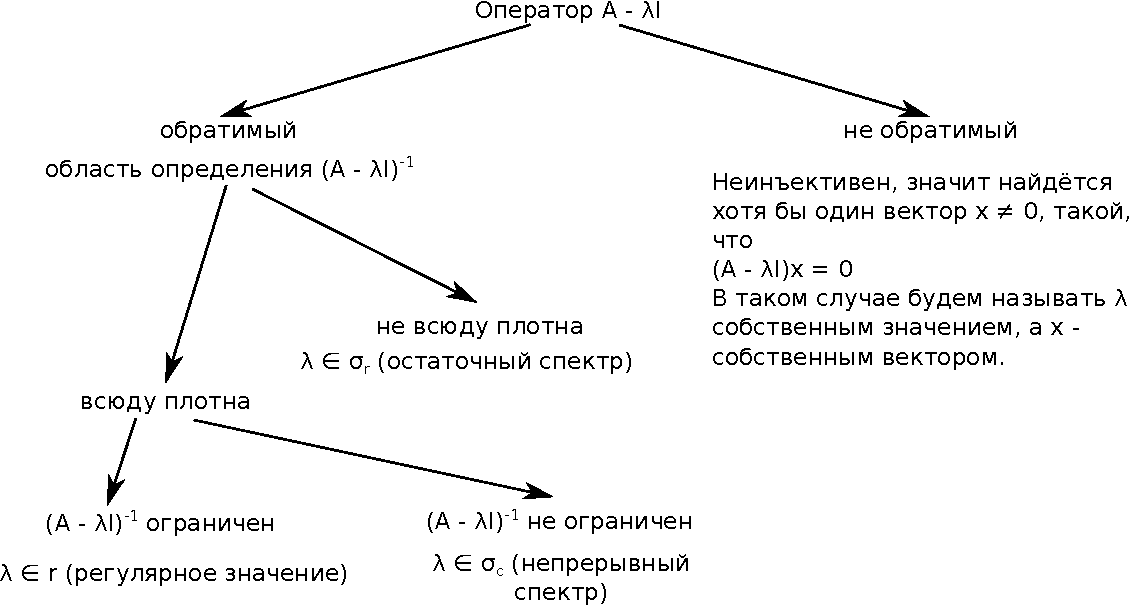
\includegraphics[width=1.0\linewidth]{../Graphics/Lectures-6-spectrum_scheme.pdf}\\
	\end{center}
	
	Для каждого $\lambda \in r(A)$ определяется ограниченный, с всюду плотной областью определения оператор
	$$ R_{\lambda} = (A - \lambda I)^{-1}$$
	Где $R_{\lambda}$ называется \textbf{резолентным оператором}. \\
	Также отметим равенство, верное для любого линейного оператора:
	$$
		\overbrace{r(A)}^{ \mathclap{\text{Регулярные значения $A$}} } \cup 
		\underbrace{\sigma_1 (A) \cup \sigma_2 (A) \cup \sigma_3 (A)}_{\text{Спектр $A$}} = 
		r(A) \cup \sigma(A) = \mathbb{C}
	$$
\end{document}
    \setcounter{section}{6}
    \documentclass[12pt]{article}

\usepackage[utf8]{inputenc}
\usepackage[russian]{babel}

\usepackage{amssymb}
\usepackage{amsmath}
\usepackage{amscd}
\usepackage{amsthm}
\usepackage{xcolor}

\usepackage{indentfirst}

%\usepackage{marginnote} % this is used for notes on the right margin --- \marginnote{\footnotesize txt}

\usepackage{mathtools} % for mathclap command

%\usepackage[normalem]{ulem} % for crossing text out - \sout

% Redefining \def is impossible. I tried, but it is impossible.
%\let\def_prev\def

%%%%%%%%%%%%%%%%%%%%%%%%%%%%%%%%%%%%%%%%%%%%%%%
%           MATH OPERATORS SPACING            %
%%%%%%%%%%%%%%%%%%%%%%%%%%%%%%%%%%%%%%%%%%%%%%%

\let\existstemp\exists
\let\foralltemp\forall
\renewcommand{\exists}{\: \existstemp \:}
\newcommand{\existsonly}{\: \existstemp ! \:}
\renewcommand{\forall}{\: \foralltemp \:}

%%%%%%%%%%%%%%%%%%%%%%%%%%%%%%%%%%%%%%%%%%%%%%%
%            COMMAND SHORTHANDS               %
%%%%%%%%%%%%%%%%%%%%%%%%%%%%%%%%%%%%%%%%%%%%%%%

\newcommand{\example}{{\itshape Пример. }}
\newcommand{\equals}{\Leftrightarrow}
\newcommand{\exc}{{\bfseries Упражнение. }}
\newcommand{\norm}[1]{\left\| #1 \right\|}
\newcommand{\scal}[2]{\left\langle #1, #2 \right\rangle}
\newcommand{\angular}[1]{\langle #1 \rangle}

\newcommand{\Sum}[2]{\underset{#1}{\overset{#2}{\sum}}}
\newcommand{\Int}[2]{\underset{#1}{\overset{#2}{\int}}}
\newcommand{\Ker}{\text{Ker}}

% Physicists' variant of dot product
\newcommand{\pscal}[2]{\, \langle #1 | #2 \rangle \,}
\newcommand{\bra}[1]{\, \langle #1 |}
\newcommand{\ket}[1]{| #1 \rangle \,}

\renewcommand{\leq}{\leqslant}
\renewcommand{\geq}{\geqslant}

%%%%%%%%%%%%%%%%%%%%%%%%%%%%%%%%%%%%%%%%%%%%%%%
%         THEOREM DEFINITION LINES            %
%%%%%%%%%%%%%%%%%%%%%%%%%%%%%%%%%%%%%%%%%%%%%%%

\newtheorem{lem}{Лемма}[section]
\newtheorem{note}{Замечание}[section]
\newtheorem{defi}{Определение}[section]
\newtheorem{theorem}{Теорема}[section]
\newtheorem{state}{Утверждение}[section] % statement

%%%%%%%%%%%%%%%%%%%%%%%%%%%%%%%%%%%%%%%%%%%%%%%
%             GRAPHICS INCLUSION              %
%%%%%%%%%%%%%%%%%%%%%%%%%%%%%%%%%%%%%%%%%%%%%%%

\usepackage{graphicx}

\graphicspath{{./Graphics/}}

%%%%%%%%%%%%%%%%%%%%%%%%%%%%%%%%%%%%%%%%%%%%%%%
%               DRAFT TEMPLATES               %
%%%%%%%%%%%%%%%%%%%%%%%%%%%%%%%%%%%%%%%%%%%%%%%

%\usepackage{marginnotes}
\newcommand{\todo}[1]{\marginpar{\color{red} \tiny #1}}

\begin{document}
	% В конспекте упущено упоминание того, что было в прошлой лекции.

	%\subsection{Спектр и регулярные значения линейного оператора}
	
	На прошлой лекции был рассмотрен оператор $(A - \lambda I)$, и классификация значений $\lambda$, определяющаяся свойствами этого 
	оператора. Для удобства, в дальнейшем будем использовать обозначение $A_{\lambda}$.
	
	\begin{state}
		Множество регулярных значений $r(A)$ оператора $A$ является открытым.
	\end{state}
	\begin{proof}
		Ранее было доказано, что оператор $(A + \Delta)$ обратим, если $\norm{\Delta} \leq \frac{1}{\norm{A^{-1}}}$ 
		и $A$ является обратимым оператором. Тогда, если $\lambda \in r(A)$, то оператор
		$$ (A - \lambda I) - \mu I $$
		является обратимым для малых $\mu$. Этим доказывается открытость множества $r(A)$.
	\end{proof}
	С другой стороны, для любого линейного оператора верно
	$$
		\overbrace{r(A)}^{ \mathclap{\text{Регулярные значения $A$}} } \cup 
		\underbrace{\sigma_1 (A) \cup \sigma_2 (A) \cup \sigma_3 (A)}_{\text{Спектр $A$}} = 
		r(A) \cup \sigma(A) = \mathbb{C}
	$$
	Данное равенство означает, что, в силу открытости $r(A)$, \textbf{спектр линейного оператора --- замкнутое множество}.
	
	\subsection*
	{
		Сопряжённые гильбертовы пространства. \\
		Основная\footnote{В рамках нашего курса.} теорема гильбертова пространства.
	}
	
	\begin{defi}
		Пусть $E$ --- банахово пространство. Тогда $E'$ будем называть 
		\textbf{пространством непрерывных линейных функционалов из $E$ в $\mathbb{C}$} 
		или \textbf{пространством, сопряжённым к $E$}.
	\end{defi}
	
	Данное определение очень похоже на определение обобщённых функций, введённых в предыдущем курсе функционального анализа. 
	Единственным отличием является то, что теперь функционалы задаются в нормированном пространстве, в отличие от
	обобщённых функций, где топология задавалась исключительно понятием сходимости
	\footnote
	{
		Строго говоря, топология пространства обобщённых функций также может определяться множеством 
		полунорм --- норм, которые могут равняться нулю на ненулевых элементах. Но эта информация выходит
		за рамки данного курса.
	}
	.
	
	Как и для линейных операторов, линейный функционал непрерывен тогда и только тогда, когда он ограничен. Единственное отличие
	между ними заключается в том, что линейные функционалы обладают фиксированным множеством прибытия.
	
	Преимущественно будем использовать $H'$ --- пространство, сопряжённое гильбертову.
	
	Рассмотрим линейный функционал $l: H \rightarrow \mathbb{C}$. Для него определено понятие ядра:
	$$\Ker(l) = \{ h \in H | l \angular{h} = 0\}$$
	В общем случае непрерывного линейного функционала, ядро обладает следующими свойствами:
	\begin{itemize}
		\item $\Ker$ --- не пустое множество. \\
		(В силу линейности в нём обязательно лежит $h = 0$)
		\item $\Ker$ --- линейное подпространство. \\
		(В силу линейности функционала)
		\item $\Ker$ --- замкнутое подпространство. \\
		(Пусть $x_n \in \Ker(l)$, $x_n \rightarrow x_0 \Rightarrow l\angular{x_n} \rightarrow l\angular{x_0}$)
	\end{itemize}
	
	\exc Доказать, что если ядро линейного функционала $f$ замкнуто, то $f$ ограничен.
	
	% TODO: Разобрать, как поставить, чтобы была не теорема 4.1, а теорема Рисса.
	\begin{theorem} 
		Пусть $l: H \rightarrow \mathbb{C}$ --- линейный ограниченнный функционал, тогда
		\begin{enumerate}
			\item $\existsonly h_l \in H$, такой, что 
			$$\forall h \in H, l \angular{h} = \scal{h}{h_l}$$
			\item $\forall g \in H$, формула (markme!) определяет линейный непрерывный функционал
			$$f\angular{h} \rightarrow \mathbb{C}$$
			$$f\angular{h} = \scal{h}{g}$$
		\end{enumerate}
	\end{theorem}
	\begin{proof}
		Докажем по порядку приведённые пункты теоремы:
		\begin{enumerate}
			\item Обозначим $G = \Ker(l)$. В таком случае, возможны два варианта:
			\begin{enumerate}
				\item Ядро совпадает с гильбертовым пространством: $(G = H)$. \\
				Данное равенство будет означать, что любой вектор пространства обращается функционалом в ноль.
				Следовательно, $h_l = 0$ будет единственным подходящим решением.
				\item Ядро не совпадает с гильбертовым пространством: $G \neq H$. \\
				Так как $G$ --- замкнутое подпространство, то его ортогональное дополнение $G^{\perp} \neq \{0\}$
				
				Тогда можно взять вектор $h_0 \in G^{\perp}, h_0 \neq 0$. Взяв произвольный $h \in H$, рассмотрим вектор
				\begin{equation} \label{eq:RissVector}
					(l\angular{h}) h_0 - (l\angular{h_0}) h
				\end{equation}
				Несложно показать, что вектор \eqref{eq:RissVector} лежит в G. Действительно,
				$$
					l\angular{(l\angular{h}) h_0 - (l\angular{h_0}) h} 
					= l\angular{h}l\angular{h_0} - l\angular{h_0}l\angular{h} = 0
				$$
				Теперь рассмотрим скалярное произведение векторов \eqref{eq:RissVector} и $h_0$:
				$$
					(l\angular{h}) \cdot \norm{h_0}^2 - (l\angular{h_0}) \cdot \scal{h}{h_0} = 0
				$$
				Откуда в результате нехитрых преобразований получается 
				\begin{equation} \label{eq:hlvector}
					h_l = \frac{\overline{l\angular{h_0}}}{\norm{h_0}^2} \cdot h_0
				\end{equation}
			\end{enumerate}
			Докажем единственность полученного $h_l$. Предположим, что это не так и существуют два вектора $h'$ и $h''$, таких, что 
			$$l\angular{h} = \scal{h}{h'} = \scal{h}{h''}$$
			Тогда будет верно
			\begin{eqnarray*}
				\scal{h}{h'} = \scal{h}{h''} \\
				\scal{h}{(h' - h'')} = 0
			\end{eqnarray*}
			Так как данное равенство верно для любых $h$, возьмём $h = h' - h''$. Получим $\norm{h'-h''}^2 = 0$, откуда следует
			$h' = h''$, что и требовалось доказать.
			
			{\footnotesize
				Единственность $h_l$ позволяет судить о размерности $G^{\perp}$.
				Так как \eqref{eq:hlvector} выполнено для всех $h_0 \in G^{\perp}$, вектор $h_l$ параллелен всем $h_0$, 
				что возможно лишь при $\dim{G^{\perp}} = 1$ ($\dim{G^{\perp}} \neq 0$ по предположению доказательства).
			}
			
			\item Рассмотрим функцию $f$, такую, что $f(h) = \scal{h}{g}$. В силу свойств скалярного произведения, 
			$f(h)$ --- линейный функционал, который, в силу неравенства Шварца, будет ограниченным:
			\begin{equation} \label{eq:BoundedProof}
				|f(h)| \leq \norm{h} \cdot \norm{g} \Rightarrow \norm{f} \leq \norm{g}
			\end{equation}
			Подставим $h = g$ в функцию $f(h)$. Получим
			$$|f(g)| = \norm{g}^2$$
			Так как норма оператора, определяется как $\sup \frac{f(h)}{\norm{h}}$, то 
			$$\norm{f} \geq \norm{g}$$
			Рассматривая данное неравенство вместе с первым неравенством из \eqref{eq:BoundedProof}, получаем 
			$$ \norm{f} = \norm{g} $$
			
			Или, в обозначениях предыдущего пункта, $\norm{h_l} = \norm{l}$.
			
			{\footnotesize
				При этом, из $\dim{G^{\perp}} \leq 1$, получим $f(h) = C(h) \cdot \norm{h}^2$, где $C(h)$ --- коэффициент из 
				\eqref{eq:hlvector}. В результате, линейный функционал для любого вектора ограничен как 
				$|f(h)| \leq C \cdot \norm{h^2}$
			}
		\end{enumerate}
	\end{proof}
	
	\begin{note}
		Теорема Рисса устанавливает биекцию $H' \leftrightarrow H$.
	\end{note}
	\begin{proof}
		Рассмотрим формулу $l_1\angular{h} = \scal{h}{h_{l_1}}, h \in H$. Для неё верны следующие
		свойства:
		\begin{itemize}
			\item Оператору $l_1 + l_2$ соответствует вектор $h_{l_1+l_2}$.
			\item Для $\alpha l_1, \alpha \in \mathbb{C}$ $h_{\alpha l_1} = \bar{\alpha} h_l$
		\end{itemize}
	\end{proof}
	
	Введя второе сопряжённое пространство $H''$, увидим следующую связь:
	$$H'' \leftrightarrow H' \leftrightarrow H$$
	При этом, здесь $\leftrightarrow$ обозначает эрмитов изоморфизм, когда 
	$h_{\alpha l} = \bar{\alpha} h_l$. % Кривовато выводит, надо будет подумать над правильной вёрсткой.
	Видим, что $H$ и $H''$ связаны обычным изоморфизмом, то есть $h_{\alpha l} = \alpha h_l$.
	% Гильбертов также называется сопряженно линейным, обычный --- канонический.
	
	\subsection{Бра- и кет-векторы.}
	Теорема Рисса отождествляет линейный ограниченный функционал с линейными вектороами гильбертова пространства.
	Но мы привыкли к префиксной записи (а здесь $h_l$, заменяющий функционал, пишется справа), поэтому у физиков
	скалярное произведение линейно по второму аргументу. На текущий и следующий разделы мы тоже <<перейдём в эту веру>>.
	
	$$\scal{f}{g} \overset{df}{=} \pscal{g}{f}$$
	Которое будем называть физическим скалярным произведением, линейным по $g$. Но мы пойдём дальше --- представив
	$\pscal{g}{f} = \bra{g} \ket{f}$, разорвём скалярное произведение. Таким образом, приходим к следующему формализму: \\
	\begin{tabular}{l c r}
		$\bra{g}$ & --- & бра-вектор \\
		$\ket{f}$ & --- & кет-вектор \\
	\end{tabular}
	(от английского \textit{bracket} --- скобки)
	
	Авторство данного формализма принадлежит Дираку, который ввёл её для описания квантовых состояний.
	
	Пусть $e_n$ --- гильбертов базис, тогда каждый вектор совпадает с суммой своего ряда Фурье:
	$$ \forall h,\quad h = \sum \alpha_n e_n,\: \alpha_n = \scal{h}{e_n} $$
	Для гильбертова базиса, запишем сначала кет-вектор, потом бра-вектор:
	$$ \ket{e_n} \bra{e_n} $$
	$$ \sum \ket{e_n} \pscal{e_n}{h_n} = \sum \ket{e_n} \alpha_n = h $$
	Так как подобное преобразование переводит $h$ в $h$, результат очевиден:
	$$ \sum \ket{e_n} \bra{e_n} = I_H $$
	
	\subsection{Операторная функция Грина}
	
	Рассмотрим линейный оператор $A : H \rightarrow H$ с собственными числами $\lambda_i$ и собственными векторами $e_i$,
	$$A e_i = \lambda_i e_i$$
	Причём $\{e_i\}$ --- гильбертов базис в $H$.
	
	Теперь рассмотрим $\lambda \neq \lambda_i$ и решим уравнение
	$$ Ax - \lambda x = y $$
	Кет-вектор $\ket{x}$ может быть записан как сумма ряда Фурье:
	$$ \ket{x} = \sum x_n \ket{e_n} $$
	Рассмотрим $A \ket{x} = \sum \lambda_n x_b \ket{e_n}$. Вычтем $\lambda \ket{x}$ из каждой стороны:
	\begin{equation} \label{ketEq}
		A\ket{x} - \lambda\ket{x} = \sum (\lambda_n - \lambda) \cdot x_ \ket{e_n} = \ket{y}
	\end{equation}
	
	Домножим \eqref{ketEq} на бра-вектор $\bra{e_m}$ слева. Тогда, так как $\{e_i\}$ --- гильбертов базис,
	то $(\lambda_n - \lambda) x_n = \pscal{e_m}{y}$.
	$$ x_m = \frac{1}{\lambda_m - \lambda} \cdot \scal{e_m}{y} $$
	Умножая полученное выражение на $\ket{e_m}$, получаем
	$$ \sum_n x_n \ket{e_m} = \sum_m \frac{\ket{e_m}}{\lambda_m - \lambda} \pscal{e_m}{y} $$
	Таким образом, получили выражение исходного вектора через результат оператора:
	$$ \ket{x} = \sum_m \frac{\ket{e_m} \bra{e_m}}{\lambda_m - \lambda} \ket{y} $$
	\begin{equation} \label{greenFunction}
		A^{-1}_{\lambda} = \sum_m \frac{\ket{e_m} \bra{e_m}}{\lambda_m - \lambda}
	\end{equation}
	Равенство \eqref{greenFunction} определяет резоленту и называется \textbf{операторной функцией Грина}.
	
	Выводя данную функцию, мы поступали как физики: не проверяли законность деления и суммирования. Но главное одно:
	результат получен.
	
	\subsection{Сопряжённые операторы}
	Рассмотрим $A: E \rightarrow F$, пусть $f\in F'$ --- линейный ограниченный функционал.
	В таком случае виден функционал $f\angular{A} \in E'$.
	
	\begin{defi} \label{def:adjointOp}
		Для линейного оператора $A: G \rightarrow F$, оператор \\$A^{*}: F' \rightarrow G'$ 
		называется \textbf{сопряжённым оператором}, если он выполняет отображение $f \mapsto g$,
		где $f \in F'$ и $g \in G'$ --- линейные функционалы, и $\forall h \in G, \: g\angular{h} = f\angular{Ah}$
	\end{defi}
	
	Тогда рассмотрим линейный ограниченный оператор $A: H_1 \rightarrow H_2 $, 
	где $H_1, H_2$ --- гильбертовы пространства. Тогда, по теореме Рисса, можем ввести
	непрерывный линейный функционал 
	$$l_2 \in H_2', \: l_2 = \scal{\:}{h_{l_2}}$$
	В таком случае, действием такого функционала на вектор $h_1 \in H_1$ будет
	$$l_2 \angular{h_1} = \scal{A h_1}{h_{l_2}}$$
	Поставим вектору $h_{l_2} \in H_2$ вектор $h_{l_1} \in H_1$, то есть
	$$ l_2 \angular{h_1} = \scal{h_1}{h_{l_1}} = \scal{h_1}{A^{*} h_{l_2}}$$
	
	По определению сопряжённого оператора, для любых $h_1 \in H_1$, $h_2 \in H_2$, будет выполняться равевнство
	\begin{equation} \label{eq:adjointOp}
		\scal{A h_1}{h_2} = \scal{h_1}{A^{*} h_2}
	\end{equation}
	
	{ \color{gray}
		Если на экзамене про сопряжённый оператор будет сказано только \eqref{eq:adjointOp}, полным <<криминалом>> это не будет.
		Тем не менее, для ответа на отличную оценку желательно сказать определение \ref{def:adjointOp}.
	}
	%%% То, что я не знаю куда запихать:
	% Гильбертов базис, в данном курсе является ортонормированной системой 
	% векоторов, которая полна.
	% В гильбертовом базисе разложение вектора по базису --- сумма ряда, в силу бесконечномерности.
	% Гильбертов базис не во всех книгах является ортонормированным.
\end{document}
\end{document}
